\documentclass[twoside]{book}

% Packages required by doxygen
\usepackage{fixltx2e}
\usepackage{calc}
\usepackage{doxygen}
\usepackage[export]{adjustbox} % also loads graphicx
\usepackage{graphicx}
\usepackage[utf8]{inputenc}
\usepackage{makeidx}
\usepackage{multicol}
\usepackage{multirow}
\PassOptionsToPackage{warn}{textcomp}
\usepackage{textcomp}
\usepackage[nointegrals]{wasysym}
\usepackage[table]{xcolor}

% Font selection
\usepackage[T1]{fontenc}
\usepackage[scaled=.90]{helvet}
\usepackage{courier}
\usepackage{amssymb}
\usepackage{sectsty}
\renewcommand{\familydefault}{\sfdefault}
\allsectionsfont{%
  \fontseries{bc}\selectfont%
  \color{darkgray}%
}
\renewcommand{\DoxyLabelFont}{%
  \fontseries{bc}\selectfont%
  \color{darkgray}%
}
\newcommand{\+}{\discretionary{\mbox{\scriptsize$\hookleftarrow$}}{}{}}

% Page & text layout
\usepackage{geometry}
\geometry{%
  a4paper,%
  top=2.5cm,%
  bottom=2.5cm,%
  left=2.5cm,%
  right=2.5cm%
}
\tolerance=750
\hfuzz=15pt
\hbadness=750
\setlength{\emergencystretch}{15pt}
\setlength{\parindent}{0cm}
\setlength{\parskip}{3ex plus 2ex minus 2ex}
\makeatletter
\renewcommand{\paragraph}{%
  \@startsection{paragraph}{4}{0ex}{-1.0ex}{1.0ex}{%
    \normalfont\normalsize\bfseries\SS@parafont%
  }%
}
\renewcommand{\subparagraph}{%
  \@startsection{subparagraph}{5}{0ex}{-1.0ex}{1.0ex}{%
    \normalfont\normalsize\bfseries\SS@subparafont%
  }%
}
\makeatother

% Headers & footers
\usepackage{fancyhdr}
\pagestyle{fancyplain}
\fancyhead[LE]{\fancyplain{}{\bfseries\thepage}}
\fancyhead[CE]{\fancyplain{}{}}
\fancyhead[RE]{\fancyplain{}{\bfseries\leftmark}}
\fancyhead[LO]{\fancyplain{}{\bfseries\rightmark}}
\fancyhead[CO]{\fancyplain{}{}}
\fancyhead[RO]{\fancyplain{}{\bfseries\thepage}}
\fancyfoot[LE]{\fancyplain{}{}}
\fancyfoot[CE]{\fancyplain{}{}}
\fancyfoot[RE]{\fancyplain{}{\bfseries\scriptsize Generated by Doxygen }}
\fancyfoot[LO]{\fancyplain{}{\bfseries\scriptsize Generated by Doxygen }}
\fancyfoot[CO]{\fancyplain{}{}}
\fancyfoot[RO]{\fancyplain{}{}}
\renewcommand{\footrulewidth}{0.4pt}
\renewcommand{\chaptermark}[1]{%
  \markboth{#1}{}%
}
\renewcommand{\sectionmark}[1]{%
  \markright{\thesection\ #1}%
}

% Indices & bibliography
\usepackage{natbib}
\usepackage[titles]{tocloft}
\setcounter{tocdepth}{3}
\setcounter{secnumdepth}{5}
\makeindex

% Hyperlinks (required, but should be loaded last)
\usepackage{ifpdf}
\ifpdf
  \usepackage[pdftex,pagebackref=true]{hyperref}
\else
  \usepackage[ps2pdf,pagebackref=true]{hyperref}
\fi
\hypersetup{%
  colorlinks=true,%
  linkcolor=blue,%
  citecolor=blue,%
  unicode%
}

% Custom commands
\newcommand{\clearemptydoublepage}{%
  \newpage{\pagestyle{empty}\cleardoublepage}%
}

\usepackage{caption}
\captionsetup{labelsep=space,justification=centering,font={bf},singlelinecheck=off,skip=4pt,position=top}

%===== C O N T E N T S =====

\begin{document}

% Titlepage & ToC
\hypersetup{pageanchor=false,
             bookmarksnumbered=true,
             pdfencoding=unicode
            }
\pagenumbering{alph}
\begin{titlepage}
\vspace*{7cm}
\begin{center}%
{\Large M\+\_\+color }\\
\vspace*{1cm}
{\large Generated by Doxygen 1.8.14}\\
\end{center}
\end{titlepage}
\clearemptydoublepage
\pagenumbering{roman}
\tableofcontents
\clearemptydoublepage
\pagenumbering{arabic}
\hypersetup{pageanchor=true}

%--- Begin generated contents ---
\chapter{M\+\_\+color Fortran Library}
\label{index}\hypertarget{index}{}    

    \hypertarget{index_Introduction}{}\section{Introduction}\label{index_Introduction}
Basic color conversion routines

      
\chapter{Modules Index}
\section{Modules List}
Here is a list of all modules with brief descriptions\+:\begin{DoxyCompactList}
\item\contentsline{section}{\mbox{\hyperlink{namespacem__color}{m\+\_\+color}} }{\pageref{namespacem__color}}{}
\end{DoxyCompactList}

\chapter{File Index}
\section{File List}
Here is a list of all files with brief descriptions\+:\begin{DoxyCompactList}
\item\contentsline{section}{/home/urbanjs/venus/\+V600/github/\+M\+\_\+color/src/\mbox{\hyperlink{M__color_8f90}{M\+\_\+color.\+f90}} }{\pageref{M__color_8f90}}{}
\end{DoxyCompactList}

\chapter{Module Documentation}
\hypertarget{namespacem__color}{}\section{m\+\_\+color Module Reference}
\label{namespacem__color}\index{m\+\_\+color@{m\+\_\+color}}
\subsection*{Functions/\+Subroutines}
\begin{DoxyCompactItemize}
\item 
subroutine, public \mbox{\hyperlink{namespacem__color_a56dd07bbf1378ccc78a230d171f9d429}{hue}} (modei, clr1i, clr2i, clr3i, modeo, clr1o, clr2o, clr3o, status)
\item 
subroutine, private \mbox{\hyperlink{namespacem__color_a1dd027cbe65112af243d26195b1fc49a}{rgbhls}} (r0, g0, b0, h, l, s, status)
\item 
subroutine, private \mbox{\hyperlink{namespacem__color_a76f00e1d418c4904a963094bc730a0e6}{rgbhvs}} (r0, g0, b0, h, v, s, status)
\item 
subroutine, private \mbox{\hyperlink{namespacem__color_ab91687e87d0901874e52efe5933e3044}{cmyrgb}} (c, m, y, r, g, b, status)
\item 
subroutine, private \mbox{\hyperlink{namespacem__color_ad6e8505eef5add299c4475d289f3c5c5}{rgbcmy}} (r, g, b, c, m, y, status)
\item 
subroutine, public \mbox{\hyperlink{namespacem__color_aca19999686fc20d79da580c6a643dc35}{rgbmono}} (rr, rg, rb, ri, status)
\begin{DoxyCompactList}\small\item\em \subsubsection*{N\+A\+ME}

R\+G\+B\+M\+O\+N\+O(3f) -\/ \mbox{[}M\+\_\+color\mbox{]} converts R\+GB colors to a reasonable grayscale intensity (L\+I\+C\+E\+N\+SE\+:PD) \end{DoxyCompactList}\item 
real function, private \mbox{\hyperlink{namespacem__color_a3e97e24dba7b820f685f13eaa64a6caa}{rgbval}} (clr1, clr2, h)
\item 
subroutine, private \mbox{\hyperlink{namespacem__color_a40e6c91da216384eded2157cdaf86eba}{hlsrgb}} (H, L, S, R, G, B, status)
\item 
subroutine, private \mbox{\hyperlink{namespacem__color_a334ec90d94bbfb9a4c08c5f9efdb8c47}{hvsrgb}} (h, v, s, r, g, b, status)
\item 
subroutine \mbox{\hyperlink{namespacem__color_ac9cd845fb9975144a6deb3a21ce29a29}{yiqrgb}} (y, i, q, r, g, b, status)
\item 
subroutine, private \mbox{\hyperlink{namespacem__color_a386d004a1392b7e01ff66f1676d43def}{rgbyiq}} (r, g, b, y, i, q, status)
\item 
subroutine, public \mbox{\hyperlink{namespacem__color_acad72628ee0b77cf87f40cd46734fb18}{closest\+\_\+color\+\_\+name}} (r, g, b, closestname)
\begin{DoxyCompactList}\small\item\em \subsubsection*{N\+A\+ME}

closest\+\_\+color\+\_\+name(3f) -\/ \mbox{[}M\+\_\+color\mbox{]} returns the closest name for the given R\+GB values. (L\+I\+C\+E\+N\+SE\+:PD) \end{DoxyCompactList}\item 
subroutine, public \mbox{\hyperlink{namespacem__color_a84a36043d278bc56a7148483a862dec8}{color\+\_\+name2rgb}} (name, r, g, b, echoname)
\begin{DoxyCompactList}\small\item\em \subsubsection*{N\+A\+ME}

C\+O\+L\+O\+R\+\_\+\+N\+A\+M\+E2\+R\+G\+B(3f) -\/ \mbox{[}M\+\_\+color\mbox{]} returns the R\+GB values in the range 0 to 100 for a given known color name. (L\+I\+C\+E\+N\+SE\+:PD) \end{DoxyCompactList}\item 
elemental pure character(len(str)) function \mbox{\hyperlink{namespacem__color_a704e93b42d777a827ec557c92d2dd7dc}{lower}} (str)
\end{DoxyCompactItemize}


\subsection{Detailed Description}

\begin{DoxyDescription}
\item[\label{_M_COLOR}%
N\+A\+ME ]

{\itshape M\+\_\+color(3fm)} -\/ \mbox{[}M\+\_\+color\mbox{]} a Fortran module that lets you convert between common color models (L\+I\+C\+E\+N\+SE\+:PD) 


\item[S\+Y\+N\+O\+P\+S\+IS ]
\begin{DoxyPre}\end{DoxyPre}



\begin{DoxyPre}    use M\_color, only : \&\end{DoxyPre}



\begin{DoxyPre}       \& \href{hue.3m_color.html}{\tt hue}, \&
       \& \href{closest_color_name.3m_color.html}{\tt closest\_color\_name}, \&
       \& \href{color_name2rgb.3m_color.html}{\tt color\_name2rgb}, \&
       \& \href{rgbmono.3m_color.html}{\tt rgbmono}
 \end{DoxyPre}
 


\item[D\+E\+S\+C\+R\+I\+P\+T\+I\+ON ]

\subsection*{Fortran color module M\+\_\+color}





Highly accurate color conversions are a tricky business, and color is a complex topic; but these simplified conversions between common color models work quite well for basic conversions. 





Typically the only user routine called is \href{hue.3m_color.html}{\tt H\+U\+E(3f)}. H\+U\+E(3f) is a single routine that interfaces to all the private low-\/level color conversion routines to convert a color\textquotesingle{}s components from one color model to another. H\+U\+E(3f) converts between the following color models\+: 




\begin{DoxyItemize}
\item R\+GB -\/ Red, Green, Blue (color TV monitors) 
\item H\+LS -\/ Hue, Lightness, Saturation 
\item C\+MY -\/ Cyan, Magenta, Yellow (pigment-\/based printing devices) 
\item H\+SV -\/ Hue, Saturation, Value 
\item Y\+IQ -\/ Broadcast TV color system 
\end{DoxyItemize}



In addition to the reversible color model conversions there are a few other user-\/callable color-\/related procedures\+: 



\href{closest_color_name.3m_color.html}{\tt C\+L\+O\+S\+E\+S\+T\+\_\+\+C\+O\+L\+O\+R\+\_\+\+N\+A\+ME}\+:~~given R\+GB values, try to find closest named color ~\newline
 \href{color_name2rgb.3m_color.html}{\tt C\+O\+L\+O\+R\+\_\+\+N\+A\+M\+E2\+R\+GB}\+:~~given a color name, return R\+GB color values in range 0 to 100 ~\newline
 \href{rgbmono.3m_color.html}{\tt R\+G\+B\+M\+O\+NO}\+:~~convert R\+GB colors to a reasonable grayscale

\paragraph*{2$\ast$N Design of the module}





The rest of the library is composed of P\+R\+I\+V\+A\+TE procedures. For each color model supported the general idea of the module is that there are two routines for each color model\+: 




\begin{DoxyItemize}
\item One converts that model to the R\+GB model  
\item The other converts from R\+GB to that model  
\end{DoxyItemize}



This allows conversions between all color models with only 2$\ast$N routines. That is, to go from model A to model B the module would internally make two calls\+: 




\begin{DoxyPre}
     call modelA2rgb(...)
     call rgb2modelB(...)
 \end{DoxyPre}




The resulting internal routines that result are\+: 




\begin{DoxyItemize}
\item \href{#HLSRGB}{\tt H\+L\+S\+R\+GB} given hue, lightness, saturation calculate red, green, and blue components 
\begin{DoxyItemize}
\item \href{#RGBVAL}{\tt R\+G\+B\+V\+AL} ensure a value is in the appropriate range and quadrant  
\end{DoxyItemize}
\item \href{#HVSRGB}{\tt H\+V\+S\+R\+GB} given hue, saturation, value calculate red, green, and blue components  
\item \href{#CMYRGB}{\tt C\+M\+Y\+R\+GB} given cyan, magenta, and yellow components calculate red, green, and blue components  
\item \href{#YIQRGB}{\tt Y\+I\+Q\+R\+GB} given luma(gray scale), orange-\/blue chrominance, and purple-\/green chrominance components calculate red, green, and blue components 


\item \href{#RGBHVS}{\tt R\+G\+B\+H\+VS} given red, green, blue values calculate hue, value, and saturation components  
\item \href{#RGBHLS}{\tt R\+G\+B\+H\+LS} given red, green, blue values calculate hue, lightness, and saturation components  
\item \href{#RGBCMY}{\tt R\+G\+B\+C\+MY} given red, green, blue values calculate cyan, magenta, yellow components  
\item \href{#RGBYIQ}{\tt R\+G\+B\+Y\+IQ} given red, green, blue values calculate luma(gray scale), orange-\/blue chrominance, and purple-\/green chrominance components 


\end{DoxyItemize}
\item[E\+X\+A\+M\+P\+LE ]

Sample program\+: 

$<$xmp$>$ program demo\+\_\+\+M\+\_\+color use M\+\_\+color, only \+: hue use M\+\_\+color, only \+: closest\+\_\+color\+\_\+name use M\+\_\+color, only \+: color\+\_\+name2rgb use M\+\_\+color, only \+: rgbmono implicit none character(len=100) \+:\+: string ! at least 20 characters character(len=20) \+:\+: name character(len=20) \+:\+: echoname real \+:\+: red,green,blue real \+:\+: gray integer \+:\+: ierr ! find the names of colors given R\+GB values write($\ast$,$\ast$)\textquotesingle{}Find names given values\textquotesingle{}

call closest\+\_\+color\+\_\+name( 100.\+0, 0.\+0, 0.\+0, string) write($\ast$,$\ast$)trim(string)

call closest\+\_\+color\+\_\+name( 0.\+0, 100.\+0, 0.\+0, string) write($\ast$,$\ast$)trim(string)

call closest\+\_\+color\+\_\+name( 0.\+0, 0.\+0, 100.\+0, string) write($\ast$,$\ast$)trim(string)

! list colors known to colorname2rgb(3f) \& corresponding R\+GB values write($\ast$,$\ast$)\textquotesingle{}given names find R\+GB values\textquotesingle{} ! get the R\+GB values and English name of the color call color\+\_\+name2rgb(\textquotesingle{}R\+ED\textquotesingle{},red,green,blue,echoname) ! display the English name and R\+GB values for the name write($\ast$,$\ast$)echoname,int(\mbox{[}red,green,blue\mbox{]})

write($\ast$,$\ast$)\textquotesingle{}Do some conversions between R\+GB, H\+LS, and H\+LS\textquotesingle{} write($\ast$,$\ast$)\textquotesingle{}and check them against expected values\textquotesingle{} ! N\+A\+ME R\+GB(0-\/255) H\+LS(0-\/100) call chk(\textquotesingle{}hls\textquotesingle{},\textquotesingle{}red\textquotesingle{}, \mbox{[}100, 0, 0 \mbox{]}, \mbox{[}0, 50, 100\mbox{]}) call chk(\textquotesingle{}hls\textquotesingle{},\textquotesingle{}orange\textquotesingle{}, \mbox{[}100, 65, 0 \mbox{]}, \mbox{[}39, 50, 100\mbox{]}) call chk(\textquotesingle{}hls\textquotesingle{},\textquotesingle{}yellow\textquotesingle{}, \mbox{[}100, 100, 0 \mbox{]}, \mbox{[}60, 50, 100\mbox{]}) call chk(\textquotesingle{}hls\textquotesingle{},\textquotesingle{}green\textquotesingle{}, \mbox{[}0, 100, 0 \mbox{]}, \mbox{[}120, 50, 100\mbox{]}) call chk(\textquotesingle{}hls\textquotesingle{},\textquotesingle{}cyan\textquotesingle{}, \mbox{[}0, 100, 100\mbox{]}, \mbox{[}180, 50, 100\mbox{]}) call chk(\textquotesingle{}hls\textquotesingle{},\textquotesingle{}blue\textquotesingle{}, \mbox{[}0, 0, 100\mbox{]}, \mbox{[}240, 50, 100\mbox{]}) call chk(\textquotesingle{}hls\textquotesingle{},\textquotesingle{}magenta\textquotesingle{}, \mbox{[}100, 0, 100\mbox{]}, \mbox{[}300, 50, 100\mbox{]}) call chk(\textquotesingle{}hls\textquotesingle{},\textquotesingle{}black\textquotesingle{}, \mbox{[}0, 0, 0 \mbox{]}, \mbox{[}0, 0, 0 \mbox{]}) call chk(\textquotesingle{}hls\textquotesingle{},\textquotesingle{}white\textquotesingle{}, \mbox{[}100, 100, 100\mbox{]}, \mbox{[}0, 100, 0 \mbox{]}) ! N\+A\+ME R\+GB(0-\/255) H\+SV(0-\/100) call chk(\textquotesingle{}hsv\textquotesingle{},\textquotesingle{}red\textquotesingle{}, \mbox{[}100, 0, 0 \mbox{]}, \mbox{[}0, 100, 100\mbox{]}) call chk(\textquotesingle{}hsv\textquotesingle{},\textquotesingle{}yellow\textquotesingle{}, \mbox{[}100, 100, 0 \mbox{]}, \mbox{[}60, 100, 100\mbox{]}) call chk(\textquotesingle{}hsv\textquotesingle{},\textquotesingle{}green\textquotesingle{}, \mbox{[}0, 100, 0 \mbox{]}, \mbox{[}120, 100, 100\mbox{]}) call chk(\textquotesingle{}hsv\textquotesingle{},\textquotesingle{}cyan\textquotesingle{}, \mbox{[}0, 100, 100\mbox{]}, \mbox{[}180, 100, 100\mbox{]}) call chk(\textquotesingle{}hsv\textquotesingle{},\textquotesingle{}blue\textquotesingle{}, \mbox{[}0, 0, 100\mbox{]}, \mbox{[}240, 100, 100\mbox{]}) call chk(\textquotesingle{}hsv\textquotesingle{},\textquotesingle{}magenta\textquotesingle{}, \mbox{[}100, 0, 100\mbox{]}, \mbox{[}300, 100, 100\mbox{]}) call chk(\textquotesingle{}hsv\textquotesingle{},\textquotesingle{}white\textquotesingle{}, \mbox{[}100, 100, 100\mbox{]}, \mbox{[}0, 0, 100\mbox{]}) call chk(\textquotesingle{}hsv\textquotesingle{},\textquotesingle{}black\textquotesingle{}, \mbox{[}0, 0, 0 \mbox{]}, \mbox{[}0, 0, 0 \mbox{]}) call chk(\textquotesingle{}hsv\textquotesingle{},\textquotesingle{}gray50\textquotesingle{}, \mbox{[}50, 50, 50 \mbox{]}, \mbox{[}0, 0, 50 \mbox{]}) call chk(\textquotesingle{}hsv\textquotesingle{},\textquotesingle{}silver\textquotesingle{}, \mbox{[}75, 75, 75 \mbox{]}, \mbox{[}0, 0, 75 \mbox{]}) call chk(\textquotesingle{}hsv\textquotesingle{},\textquotesingle{}red4\textquotesingle{}, \mbox{[}55, 0, 0 \mbox{]}, \mbox{[}0, 100, 55 \mbox{]}) call chk(\textquotesingle{}hsv\textquotesingle{},\textquotesingle{}olive\textquotesingle{}, \mbox{[}50, 50, 0 \mbox{]}, \mbox{[}60, 100, 50 \mbox{]}) call chk(\textquotesingle{}hsv\textquotesingle{},\textquotesingle{}lime\textquotesingle{}, \mbox{[}0, 100, 0 \mbox{]}, \mbox{[}120, 100, 100\mbox{]}) call chk(\textquotesingle{}hsv\textquotesingle{},\textquotesingle{}teal\textquotesingle{}, \mbox{[}0, 50, 50 \mbox{]}, \mbox{[}180, 100, 50 \mbox{]}) call chk(\textquotesingle{}hsv\textquotesingle{},\textquotesingle{}navy\textquotesingle{}, \mbox{[}0, 0, 50 \mbox{]}, \mbox{[}240, 100, 50 \mbox{]}) call chk(\textquotesingle{}hsv\textquotesingle{},\textquotesingle{}purple\textquotesingle{}, \mbox{[}63, 13, 94 \mbox{]}, \mbox{[}277, 87, 94 \mbox{]}) call chk(\textquotesingle{}hsv\textquotesingle{},\textquotesingle{}magenta4\textquotesingle{},\mbox{[}55, 0, 55 \mbox{]}, \mbox{[}300, 100, 55 \mbox{]}) call chk(\textquotesingle{}hsv\textquotesingle{},\textquotesingle{}maroon\textquotesingle{}, \mbox{[}69, 19, 38 \mbox{]}, \mbox{[}338, 73, 69 \mbox{]})

write($\ast$,$\ast$)\textquotesingle{}Get some grayscale values from R\+GB color values\textquotesingle{} call rgbmono(100.\+0, 0.\+0, 0.\+0,gray,ierr); write($\ast$,$\ast$)\textquotesingle{}red \textquotesingle{},gray call rgbmono( 0.\+0,100.\+0, 0.\+0,gray,ierr); write($\ast$,$\ast$)\textquotesingle{}green \textquotesingle{},gray call rgbmono( 0.\+0, 0.\+0,100.\+0,gray,ierr); write($\ast$,$\ast$)\textquotesingle{}blue \textquotesingle{},gray call rgbmono(100.\+0,100.\+0, 0.\+0,gray,ierr); write($\ast$,$\ast$)\textquotesingle{}Yellow \textquotesingle{},gray call rgbmono( 0.\+0,100.\+0,100.\+0,gray,ierr); write($\ast$,$\ast$)\textquotesingle{}Cyan \textquotesingle{},gray call rgbmono(100.\+0, 0.\+0,100.\+0,gray,ierr); write($\ast$,$\ast$)\textquotesingle{}Magenta \textquotesingle{},gray call rgbmono(100.\+0,100.\+0,100.\+0,gray,ierr); write($\ast$,$\ast$)\textquotesingle{}White \textquotesingle{},gray call rgbmono( 00.\+0, 0.\+0, 0.\+0,gray,ierr); write($\ast$,$\ast$)\textquotesingle{}Black \textquotesingle{},gray call rgbmono( 50.\+0, 0.\+0, 0.\+0,gray,ierr); write($\ast$,$\ast$)\textquotesingle{}Maroon \textquotesingle{},gray call rgbmono(100.\+0, 50.\+0, 50.\+0,gray,ierr); write($\ast$,$\ast$)\textquotesingle{}Pink \textquotesingle{},gray contains subroutine chk(modelout,name,rgb,other) ! given a color convert to M\+O\+D\+E\+L\+O\+UT and compare to expected values character(len=$\ast$),intent(in) \+:\+: name integer,intent(in) \+:\+: rgb(3), other(3) character(len=$\ast$),intent(in) \+:\+: modelout real \+:\+: val1,val2,val3 integer \+:\+: status ! convert R\+GB values to M\+O\+D\+E\+L\+O\+UT values call hue(\textquotesingle{}rgb\textquotesingle{},R\+E\+A\+L(rgb(1)),R\+E\+A\+L(rgb(2)),R\+E\+A\+L(rgb(3)),\& \& modelout,val1,val2,val3,status) ! left-\/justify name to 10 characters or more write($\ast$,\textquotesingle{}(a,1x)\textquotesingle{},advance=\textquotesingle{}no\textquotesingle{}) \& \& \mbox{[} character(len=max(10,len\+\_\+trim(name))) \+:\+:\textquotesingle{} \textquotesingle{}//trim(name)\mbox{]} write($\ast$,\textquotesingle{}(a,1x,3(i3,1x))\textquotesingle{},advance=\textquotesingle{}no\textquotesingle{}) \& \& modelout//\textquotesingle{} E\+X\+P\+E\+C\+T\+ED\textquotesingle{},other write($\ast$,\textquotesingle{}(a,1x,3(i3,1x))\textquotesingle{},advance=\textquotesingle{}no\textquotesingle{}) \& \& \textquotesingle{}G\+OT\textquotesingle{},int(\mbox{[}val1+0.5,val2+0.5,val3+0.5\mbox{]}) write($\ast$,\textquotesingle{}(a,i0)\textquotesingle{})\textquotesingle{}S\+T\+A\+T\+US \textquotesingle{},status end subroutine chk end program demo\+\_\+\+M\+\_\+color $<$/xmp$>$ 


\item[S\+EE A\+L\+SO  ]



A simple interactive javascript-\/based \href{../../../public_html/javascript/color/iframe.html}{\tt color selector} lets you interactively select colors. 





The color wheel below was generated using a \href{BOOK_M_draw.html}{\tt M\+\_\+draw(3f) } graphics library program \href{../test/demos/huegif.f90}{\tt (huegif.\+f90)} that uses the M\+\_\+color module. 



\begin{center}  \end{center} 




\item[R\+E\+F\+E\+R\+E\+N\+C\+ES]The algorithms are based on chapter 17 of \char`\"{}\+Fundamentals of Interactive Computer Graphics\char`\"{}; J. D. Foley and A. Van Dam. 


\item[A\+U\+T\+H\+OR ]

John S. Urban




\item[L\+I\+C\+E\+N\+SE ]

Public Domain




\end{DoxyDescription}

\subsection{Function/\+Subroutine Documentation}
\mbox{\Hypertarget{namespacem__color_acad72628ee0b77cf87f40cd46734fb18}\label{namespacem__color_acad72628ee0b77cf87f40cd46734fb18}} 
\index{m\+\_\+color@{m\+\_\+color}!closest\+\_\+color\+\_\+name@{closest\+\_\+color\+\_\+name}}
\index{closest\+\_\+color\+\_\+name@{closest\+\_\+color\+\_\+name}!m\+\_\+color@{m\+\_\+color}}
\subsubsection{\texorpdfstring{closest\+\_\+color\+\_\+name()}{closest\_color\_name()}}
{\footnotesize\ttfamily subroutine, public m\+\_\+color\+::closest\+\_\+color\+\_\+name (\begin{DoxyParamCaption}\item[{real, intent(in)}]{r,  }\item[{real, intent(in)}]{g,  }\item[{real, intent(in)}]{b,  }\item[{character(len=$\ast$), intent(out)}]{closestname }\end{DoxyParamCaption})}



\subsubsection*{N\+A\+ME}

closest\+\_\+color\+\_\+name(3f) -\/ \mbox{[}M\+\_\+color\mbox{]} returns the closest name for the given R\+GB values. (L\+I\+C\+E\+N\+SE\+:PD) 

\subsubsection*{S\+Y\+N\+O\+P\+S\+IS}

\begin{DoxyVerb}subroutine closest_color_name(r,g,b,closestname)

 real,intent(in)               :: r,g,b
 character(len=20),intent(out) :: closestname
\end{DoxyVerb}


\subsubsection*{D\+E\+S\+C\+R\+I\+P\+T\+I\+ON}

\mbox{\hyperlink{namespacem__color_acad72628ee0b77cf87f40cd46734fb18}{closest\+\_\+color\+\_\+name()}} returns the closest name for the given R\+GB values. Most X11 Windows color names are supported.

\subsubsection*{O\+P\+T\+I\+O\+NS}

R red component, range of 0 to 100 G green component, range of 0 to 100 B blue component, range of 0 to 100

\subsubsection*{R\+E\+T\+U\+R\+NS}

C\+L\+O\+S\+E\+S\+T\+N\+A\+ME name of color found closest to given R\+GB value

\subsubsection*{E\+X\+A\+M\+P\+LE}

Sample program

program demo\+\_\+closest\+\_\+color\+\_\+name use M\+\_\+color, only \+: closest\+\_\+color\+\_\+name character(len=100) \+:\+: string ! at least 20 characters string=\textquotesingle{} \textquotesingle{}

call closest\+\_\+color\+\_\+name(100.\+0, 0.\+0, 0.\+0,string) write($\ast$,$\ast$)trim(string)

call closest\+\_\+color\+\_\+name( 0.\+0,100.\+0, 0.\+0,string) write($\ast$,$\ast$)trim(string)

call closest\+\_\+color\+\_\+name( 0.\+0, 0.\+0,100.\+0,string) write($\ast$,$\ast$)trim(string)

end program demo\+\_\+closest\+\_\+color\+\_\+name

Results\+:

red green blue

\subsubsection*{A\+U\+T\+H\+OR}

John S. Urban

\subsubsection*{L\+I\+C\+E\+N\+SE}

Public Domain 

References color\+\_\+name2rgb().

Here is the call graph for this function\+:\nopagebreak
\begin{figure}[H]
\begin{center}
\leavevmode
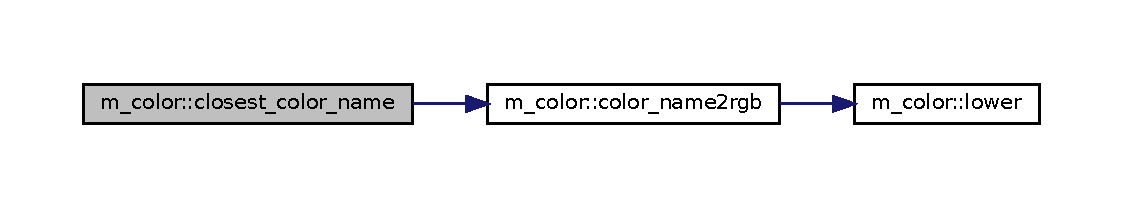
\includegraphics[width=350pt]{namespacem__color_acad72628ee0b77cf87f40cd46734fb18_cgraph}
\end{center}
\end{figure}
\mbox{\Hypertarget{namespacem__color_ab91687e87d0901874e52efe5933e3044}\label{namespacem__color_ab91687e87d0901874e52efe5933e3044}} 
\index{m\+\_\+color@{m\+\_\+color}!cmyrgb@{cmyrgb}}
\index{cmyrgb@{cmyrgb}!m\+\_\+color@{m\+\_\+color}}
\subsubsection{\texorpdfstring{cmyrgb()}{cmyrgb()}}
{\footnotesize\ttfamily subroutine, private m\+\_\+color\+::cmyrgb (\begin{DoxyParamCaption}\item[{real, intent(in)}]{c,  }\item[{real, intent(in)}]{m,  }\item[{real, intent(in)}]{y,  }\item[{real, intent(out)}]{r,  }\item[{real, intent(out)}]{g,  }\item[{real, intent(out)}]{b,  }\item[{integer}]{status }\end{DoxyParamCaption})\hspace{0.3cm}{\ttfamily [private]}}


\begin{DoxyDescription}
\item[\label{_CMYRGB}%
N\+A\+ME ]cmyrgb(3fp) -\/ \mbox{[}M\+\_\+color\mbox{]} calculates the cyan, magenta, and yellow components given the red, green, and blue component values. (L\+I\+C\+E\+N\+SE\+:PD) 


\item[S\+Y\+N\+O\+P\+S\+IS ]
\begin{DoxyPre}
    subroutine cmyrgb(c,m,y,r,g,b,status)\end{DoxyPre}



\begin{DoxyPre}     ! cyan component as a value in the range of 0 to 100
     real, intent(in)  :: c
     ! magenta component as a value in the range of 0 to 100
     real, intent(in)  :: m
     ! yellow component as a value in the range of 0 to 100
     real, intent(in)  :: y
     ! red component as a value in the range of 0 to 100
     real, intent(out) :: r
     ! green component as a value in the range of 0 to 100
     real, intent(out) :: g
     ! blue component as a value in the range of 0 to 100
     real, intent(out) :: b
     integer           :: status
    \end{DoxyPre}
 


\item[D\+E\+S\+C\+R\+I\+P\+T\+I\+ON ]\mbox{\hyperlink{namespacem__color_ab91687e87d0901874e52efe5933e3044}{cmyrgb()}} calculates the cyan, magenta, and yellow components given the red, green, and blue component values.




\item[A\+U\+T\+H\+OR ]

John S. Urban




\item[L\+I\+C\+E\+N\+SE ]

Public Domain




\end{DoxyDescription}Here is the caller graph for this function\+:\nopagebreak
\begin{figure}[H]
\begin{center}
\leavevmode
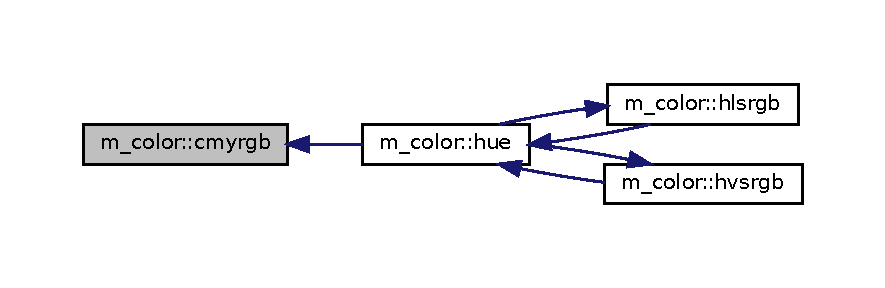
\includegraphics[width=350pt]{namespacem__color_ab91687e87d0901874e52efe5933e3044_icgraph}
\end{center}
\end{figure}
\mbox{\Hypertarget{namespacem__color_a84a36043d278bc56a7148483a862dec8}\label{namespacem__color_a84a36043d278bc56a7148483a862dec8}} 
\index{m\+\_\+color@{m\+\_\+color}!color\+\_\+name2rgb@{color\+\_\+name2rgb}}
\index{color\+\_\+name2rgb@{color\+\_\+name2rgb}!m\+\_\+color@{m\+\_\+color}}
\subsubsection{\texorpdfstring{color\+\_\+name2rgb()}{color\_name2rgb()}}
{\footnotesize\ttfamily subroutine, public m\+\_\+color\+::color\+\_\+name2rgb (\begin{DoxyParamCaption}\item[{character(len=$\ast$), intent(in)}]{name,  }\item[{real, intent(out)}]{r,  }\item[{real, intent(out)}]{g,  }\item[{real, intent(out)}]{b,  }\item[{character(len=$\ast$), intent(out), optional}]{echoname }\end{DoxyParamCaption})}



\subsubsection*{N\+A\+ME}

C\+O\+L\+O\+R\+\_\+\+N\+A\+M\+E2\+R\+G\+B(3f) -\/ \mbox{[}M\+\_\+color\mbox{]} returns the R\+GB values in the range 0 to 100 for a given known color name. (L\+I\+C\+E\+N\+SE\+:PD) 

\subsubsection*{S\+Y\+N\+O\+P\+S\+IS}

\begin{DoxyVerb}subroutine color_name2rgb(name,r,g,b,echoname)

 character(len=20),intent(in)   :: name
 real,intent(out)               :: r,g,b
 character(len=20),intent(out)  :: echoname
\end{DoxyVerb}


\subsubsection*{D\+E\+S\+C\+R\+I\+P\+T\+I\+ON}

C\+O\+L\+O\+R\+\_\+\+N\+A\+M\+E2\+R\+G\+B() returns the R\+GB values in the range 0 to 100 for a given known color name. Most X11 Windows color names are supported. If the name is not found, E\+C\+H\+O\+N\+A\+ME is set to \char`\"{}\+Unknown\char`\"{}.

\subsubsection*{E\+X\+A\+M\+P\+LE}

\begin{DoxyVerb}A sample program:

 program demo_color_name2rgb
 use M_color, only : hue, color_name2rgb
 implicit none
 !
 ! list colors known to colorname2rgb(3f) & corresponding RGB values
 !
 character(len=20) :: name
 character(len=20) :: echoname
 real              :: red,green,blue
 integer           :: i
 TRYALL: do i=1,10000
    ! weird little thing where the color names have aliases
    ! that are numeric strings
    write(name,'(i0)')i
    ! get the RGB values and English name of the color
    call color_name2rgb(name,red,green,blue,echoname)
    ! the last color name is "Unknown" so the loop should exit
    if(echoname.eq.'Unknown')exit TRYALL
    ! display the English name and RGB values for the name
    write(*,*)echoname,int([red,green,blue])
 enddo TRYALL
 !write(*,*)'Number of colors found is ',i-1
 end program demo_color_name2rgb
\end{DoxyVerb}


\subsubsection*{A\+U\+T\+H\+OR}

John S. Urban

\subsubsection*{L\+I\+C\+E\+N\+SE}

Public Domain 

References lower().

Here is the call graph for this function\+:\nopagebreak
\begin{figure}[H]
\begin{center}
\leavevmode
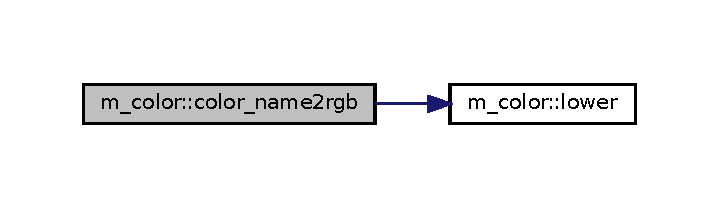
\includegraphics[width=345pt]{namespacem__color_a84a36043d278bc56a7148483a862dec8_cgraph}
\end{center}
\end{figure}
Here is the caller graph for this function\+:\nopagebreak
\begin{figure}[H]
\begin{center}
\leavevmode
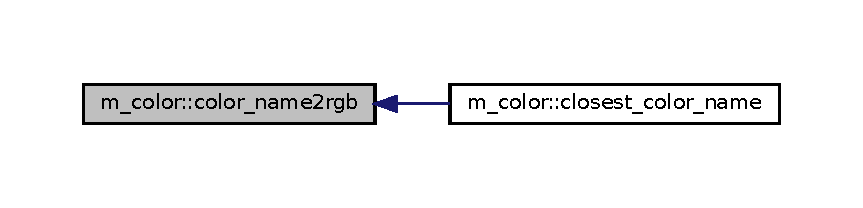
\includegraphics[width=350pt]{namespacem__color_a84a36043d278bc56a7148483a862dec8_icgraph}
\end{center}
\end{figure}
\mbox{\Hypertarget{namespacem__color_a40e6c91da216384eded2157cdaf86eba}\label{namespacem__color_a40e6c91da216384eded2157cdaf86eba}} 
\index{m\+\_\+color@{m\+\_\+color}!hlsrgb@{hlsrgb}}
\index{hlsrgb@{hlsrgb}!m\+\_\+color@{m\+\_\+color}}
\subsubsection{\texorpdfstring{hlsrgb()}{hlsrgb()}}
{\footnotesize\ttfamily subroutine, private m\+\_\+color\+::hlsrgb (\begin{DoxyParamCaption}\item[{real, intent(in)}]{H,  }\item[{real, intent(in)}]{L,  }\item[{real, intent(in)}]{S,  }\item[{real, intent(out)}]{R,  }\item[{real, intent(out)}]{G,  }\item[{real, intent(out)}]{B,  }\item[{integer}]{status }\end{DoxyParamCaption})\hspace{0.3cm}{\ttfamily [private]}}


\begin{DoxyDescription}
\item[\label{_HLSRGB}%
N\+A\+ME ]H\+L\+S\+R\+G\+B(3fp) -\/ \mbox{[}M\+\_\+color\mbox{]} calculates the red, green, \& blue components for a color given in hue, lightness, \& saturation values. (L\+I\+C\+E\+N\+SE\+:PD) 


\item[S\+Y\+N\+O\+P\+S\+IS ]
\begin{DoxyPre}
    subroutine hlsrgb (h,l,s,r,g,b,status)\end{DoxyPre}



\begin{DoxyPre}     ! hue value in the range of 0 to 360 degrees
     real, intent(in)  :: h
     ! lightness as a percent value from 0 to 100.
     real, intent(in)  :: l
     ! saturation as a percent from 0 to 100.
     real, intent(in)  :: s
     ! red component as a value of 0 to 100.
     real, intent(out) :: r
     ! green component as a value of 0 to 100.
     real, intent(out) :: g
     ! blue component as a value of 0 to 100.
     real, intent(out) :: b
     integer           :: status
    \end{DoxyPre}
 


\item[D\+E\+S\+C\+R\+I\+P\+T\+I\+ON ]\begin{DoxyVerb}HLSRGB() calculates the red, green, &amp; blue components for a
 color given in hue, lightness, &amp; saturation values.
\end{DoxyVerb}
 


\item[A\+U\+T\+H\+OR ]

John S. Urban




\item[L\+I\+C\+E\+N\+SE ]

Public Domain




\end{DoxyDescription}

References hue(), and rgbval().

Here is the call graph for this function\+:\nopagebreak
\begin{figure}[H]
\begin{center}
\leavevmode
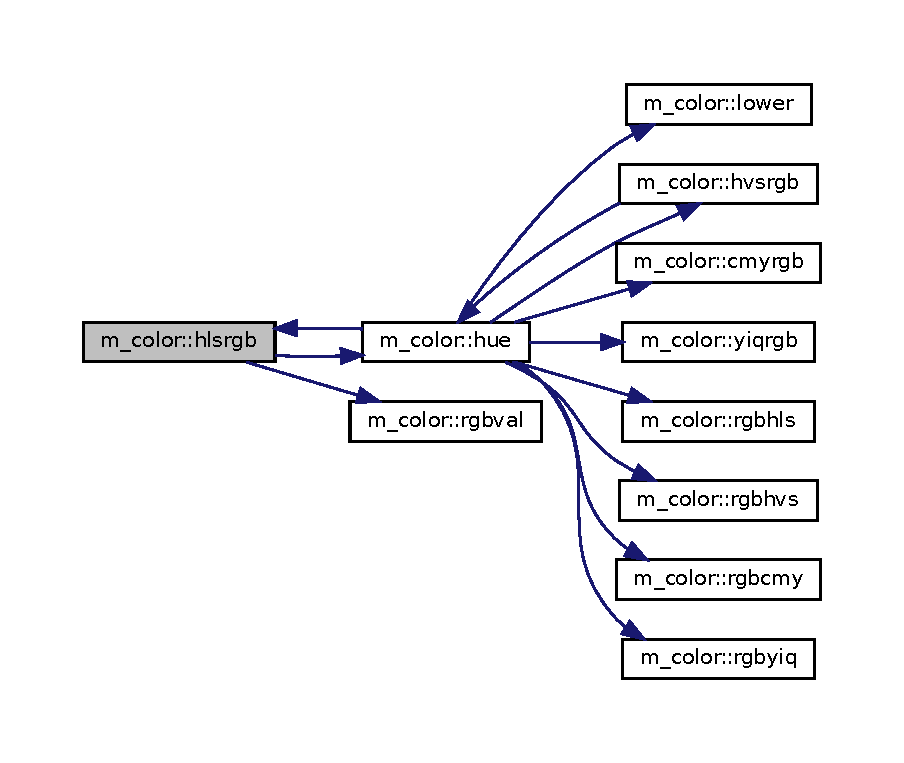
\includegraphics[width=350pt]{namespacem__color_a40e6c91da216384eded2157cdaf86eba_cgraph}
\end{center}
\end{figure}
Here is the caller graph for this function\+:\nopagebreak
\begin{figure}[H]
\begin{center}
\leavevmode
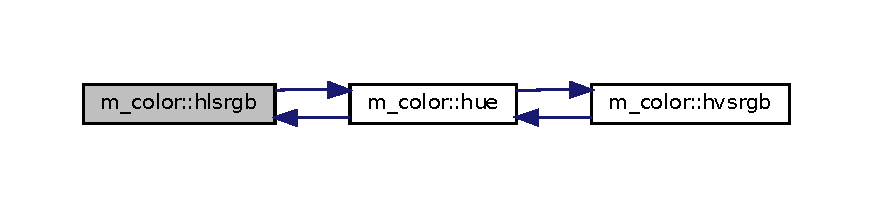
\includegraphics[width=350pt]{namespacem__color_a40e6c91da216384eded2157cdaf86eba_icgraph}
\end{center}
\end{figure}
\mbox{\Hypertarget{namespacem__color_a56dd07bbf1378ccc78a230d171f9d429}\label{namespacem__color_a56dd07bbf1378ccc78a230d171f9d429}} 
\index{m\+\_\+color@{m\+\_\+color}!hue@{hue}}
\index{hue@{hue}!m\+\_\+color@{m\+\_\+color}}
\subsubsection{\texorpdfstring{hue()}{hue()}}
{\footnotesize\ttfamily subroutine, public m\+\_\+color\+::hue (\begin{DoxyParamCaption}\item[{character(len=$\ast$), intent(in)}]{modei,  }\item[{real, intent(in)}]{clr1i,  }\item[{real, intent(in)}]{clr2i,  }\item[{real, intent(in)}]{clr3i,  }\item[{character(len=$\ast$), intent(in)}]{modeo,  }\item[{real, intent(out)}]{clr1o,  }\item[{real, intent(out)}]{clr2o,  }\item[{real, intent(out)}]{clr3o,  }\item[{integer, intent(out)}]{status }\end{DoxyParamCaption})}


\begin{DoxyDescription}
\item[\label{_HUE}%
N\+A\+ME ]H\+U\+E(3f) -\/ \mbox{[}M\+\_\+color\mbox{]} converts a color\textquotesingle{}s components from one color model to another. (L\+I\+C\+E\+N\+SE\+:PD) 


\item[S\+Y\+N\+O\+P\+S\+IS ]
\begin{DoxyPre}
 subroutine hue(modei,clr1i,clr2i,clr3i,modeo,clr1o,clr2o,clr3o,status)\end{DoxyPre}



\begin{DoxyPre}  character(len=*),intent(in) :: modei  ! color model of input values
  character(len=*),intent(in) :: modeo  ! color model of output values
  real,intent(in)             :: clr1i,clr2i,clr3i
  real,intent(out)            :: clr1o,clr2o,clr3o
  integer,intent(out)         :: status
 \end{DoxyPre}
 


\item[D\+E\+S\+C\+R\+I\+P\+T\+I\+ON ]
\item[Basic color models ..]

Valid values for modei and modeo as well as the corresponding meanings for clr1$\ast$, clr2$\ast$, and clr3$\ast$ are\+:

\tabulinesep=1mm
\begin{longtabu} spread 0pt [c]{*{4}{|X[-1]}|}
\hline
\rowcolor{\tableheadbgcolor}\textbf{ model}&\textbf{ clr1 }&\textbf{ clr2 }&\textbf{ clr3  }\\\cline{1-4}
\endfirsthead
\hline
\endfoot
\hline
\rowcolor{\tableheadbgcolor}\textbf{ model}&\textbf{ clr1 }&\textbf{ clr2 }&\textbf{ clr3  }\\\cline{1-4}
\endhead
hls &hue &lightness &saturation \\\cline{1-4}
hsl &hue &saturation&lightness  \\\cline{1-4}
hvs &hue &value &saturation \\\cline{1-4}
hsv &hue &saturation&value  \\\cline{1-4}
rgb &red &green &blue  \\\cline{1-4}
cmy &cyan &magenta &yellow  \\\cline{1-4}
yiq &luma grayscale &orange-\/bluechrominance &purple-\/greenchrominance  \\\cline{1-4}
\end{longtabu}





\begin{DoxyItemize}
\item lightness, value, saturation, red, green, blue, cyan, magenta, and yellow range from 0 to 100, 
\item hue ranges from 0 to 360 degrees, 
\item y ranges from 0 to 100, 
\item i ranges from -\/60 to 60, 
\item q ranges from -\/52 to 52 
\end{DoxyItemize}



The S\+T\+A\+T\+US variable can signal the following conditions\+: 




\begin{DoxyPre}\end{DoxyPre}



\begin{DoxyPre}    -1   modei = modeo, so no substantial conversion was done,
     1   one of the input color values was outside the allowable range,
     2   modei was invalid
     3   modeo was invalid
 \end{DoxyPre}
 \subsubsection*{E\+X\+A\+M\+P\+LE}


\begin{DoxyPre}\end{DoxyPre}



\begin{DoxyPre}   Sample program\end{DoxyPre}



\begin{DoxyPre}    program demo\_hue
    use M\_color, only : hue
    implicit none
       !               NAME        RGB(0-255)            HLS(0-100)
       call chk('hls','red',     [100, 0,   0  ], [0,   50,  100])
       call chk('hls','orange',  [100, 65,  0  ], [39,  50,  100])
       call chk('hls','yellow',  [100, 100, 0  ], [60,  50,  100])
       call chk('hls','green',   [0,   100, 0  ], [120, 50,  100])
       call chk('hls','cyan',    [0,   100, 100], [180, 50,  100])
       call chk('hls','blue',    [0,   0,   100], [240, 50,  100])
       call chk('hls','magenta', [100, 0,   100], [300, 50,  100])
       call chk('hls','black',   [0,   0,   0  ], [0,   0,   0  ])
       call chk('hls','white',   [100, 100, 100], [0,   100, 0  ])
       !               NAME        RGB(0-255)           HSV(0-100)
       call chk('hsv','red',     [100, 0,   0  ], [0,   100, 100])
       call chk('hsv','yellow',  [100, 100, 0  ], [60,  100, 100])
       call chk('hsv','green',   [0,   100, 0  ], [120, 100, 100])
       call chk('hsv','cyan',    [0,   100, 100], [180, 100, 100])
       call chk('hsv','blue',    [0,   0,   100], [240, 100, 100])
       call chk('hsv','magenta', [100, 0,   100], [300, 100, 100])
       call chk('hsv','black',   [0,   0,   0  ], [0,   0,   0  ])
       call chk('hsv','white',   [100, 100, 100], [0,   0,   100])\end{DoxyPre}



\begin{DoxyPre}       call chk('hsv','gray50',  [50,  50,  50 ], [0,   0,   50 ])
       call chk('hsv','silver',  [75,  75,  75 ], [0,   0,   75 ])
       call chk('hsv','red4',    [55,  0,   0  ], [0,   100, 55 ])
       call chk('hsv','olive',   [50,  50,  0  ], [60,  100, 50 ])
       call chk('hsv','lime',    [0,   100, 0  ], [120, 100, 100])
       call chk('hsv','teal',    [0,   50,  50 ], [180, 100, 50 ])
       call chk('hsv','navy',    [0,   0,   50 ], [240, 100, 50 ])
       call chk('hsv','purple',  [63,  13,  94 ], [277, 87,  94 ])
       call chk('hsv','magenta4',[55,  0,   55 ], [300, 100, 55 ])
       call chk('hsv','maroon',  [69,  19,  38 ], [338, 73,  69 ])
    contains
    subroutine chk(modelout,name,rgb,other)
    ! given a color convert to MODELOUT and compare to expected values
    character(len=*),intent(in)   :: name
    integer,intent(in)            :: rgb(3), other(3)
    character(len=*),intent(in)   :: modelout
       real                       :: val1,val2,val3
       integer                    :: status
       ! convert RGB values to MODELOUT values
       call hue('rgb',REAL(rgb(1)),REAL(rgb(2)),REAL(rgb(3)),\&
       \& modelout,val1,val2,val3,status)
          ! left-justify name to 10 characters or more
          write(*,'(a,1x)',advance='no') \&
          \& [ character(len=max(10,len\_trim(name))) ::' '//trim(name)]
          write(*,'(a,1x,3(i3,1x))',advance='no') \&
          \& modelout//' EXPECTED',other
          write(*,'(a,1x,3(i3,1x))',advance='no') \&
          \& 'GOT',int([val1+0.5,val2+0.5,val3+0.5])
          write(*,'(a,i0)')'STATUS ',status
    end subroutine chk
    end program demo\_hue\end{DoxyPre}



\begin{DoxyPre}   Results:\end{DoxyPre}



\begin{DoxyPre}     red       hls EXPECTED   0  50 100 GOT   0  50 100 STATUS 0
     orange    hls EXPECTED  39  50 100 GOT  39  50 100 STATUS 0
     yellow    hls EXPECTED  60  50 100 GOT  60  50 100 STATUS 0
     green     hls EXPECTED 120  50 100 GOT 120  50 100 STATUS 0
     cyan      hls EXPECTED 180  50 100 GOT 180  50 100 STATUS 0
     blue      hls EXPECTED 240  50 100 GOT 240  50 100 STATUS 0
     magenta   hls EXPECTED 300  50 100 GOT 300  50 100 STATUS 0
     black     hls EXPECTED   0   0   0 GOT   0   0   0 STATUS 0
     white     hls EXPECTED   0 100   0 GOT   0 100   0 STATUS 0
     black     hsv EXPECTED   0   0   0 GOT   0   0   0 STATUS 0
     gray50    hsv EXPECTED   0   0  50 GOT   0   0  50 STATUS 0
     silver    hsv EXPECTED   0   0  75 GOT   0   0  75 STATUS 0
     white     hsv EXPECTED   0   0 100 GOT   0   0 100 STATUS 0
     red4      hsv EXPECTED   0 100  55 GOT   0 100  55 STATUS 0
     red       hsv EXPECTED   0 100 100 GOT   0 100 100 STATUS 0
     olive     hsv EXPECTED  60 100  50 GOT  60 100  50 STATUS 0
     yellow    hsv EXPECTED  60 100 100 GOT  60 100 100 STATUS 0
     green     hsv EXPECTED 120 100 100 GOT 120 100 100 STATUS 0
     lime      hsv EXPECTED 120 100 100 GOT 120 100 100 STATUS 0
     teal      hsv EXPECTED 180 100  50 GOT 180 100  50 STATUS 0
     cyan      hsv EXPECTED 180 100 100 GOT 180 100 100 STATUS 0
     navy      hsv EXPECTED 240 100  50 GOT 240 100  50 STATUS 0
     blue      hsv EXPECTED 240 100 100 GOT 240 100 100 STATUS 0
     purple    hsv EXPECTED 277  87  94 GOT 277  86  94 STATUS 0
     magenta4  hsv EXPECTED 300 100  55 GOT 300 100  55 STATUS 0
     magenta   hsv EXPECTED 300 100 100 GOT 300 100 100 STATUS 0
     maroon    hsv EXPECTED 338  73  69 GOT 337  72  69 STATUS 0
 \end{DoxyPre}
 


\item[A\+U\+T\+H\+OR ]

John S. Urban




\item[L\+I\+C\+E\+N\+SE ]

Public Domain




\end{DoxyDescription}

References cmyrgb(), hlsrgb(), hvsrgb(), lower(), rgbcmy(), rgbhls(), rgbhvs(), rgbyiq(), and yiqrgb().

Here is the call graph for this function\+:\nopagebreak
\begin{figure}[H]
\begin{center}
\leavevmode
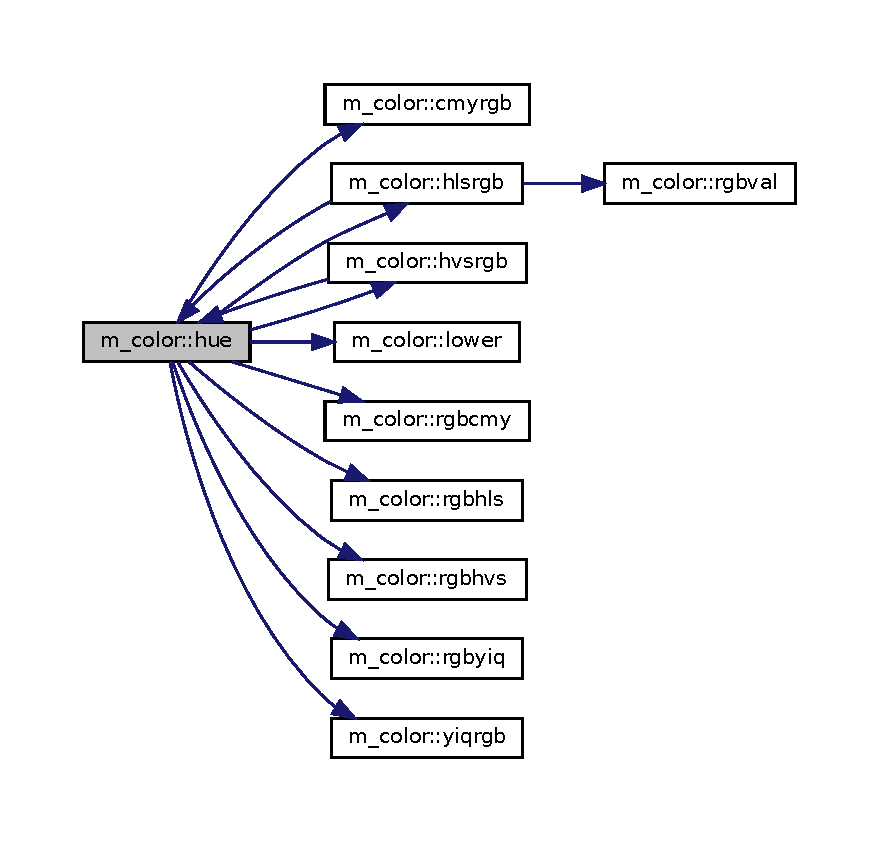
\includegraphics[width=350pt]{namespacem__color_a56dd07bbf1378ccc78a230d171f9d429_cgraph}
\end{center}
\end{figure}
Here is the caller graph for this function\+:\nopagebreak
\begin{figure}[H]
\begin{center}
\leavevmode
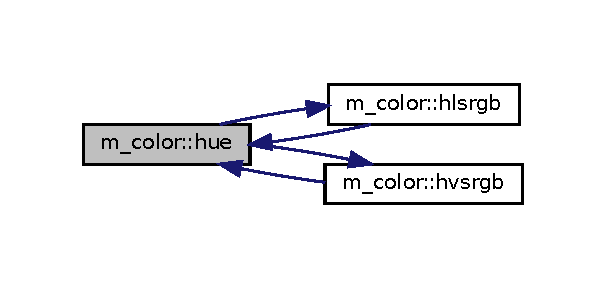
\includegraphics[width=291pt]{namespacem__color_a56dd07bbf1378ccc78a230d171f9d429_icgraph}
\end{center}
\end{figure}
\mbox{\Hypertarget{namespacem__color_a334ec90d94bbfb9a4c08c5f9efdb8c47}\label{namespacem__color_a334ec90d94bbfb9a4c08c5f9efdb8c47}} 
\index{m\+\_\+color@{m\+\_\+color}!hvsrgb@{hvsrgb}}
\index{hvsrgb@{hvsrgb}!m\+\_\+color@{m\+\_\+color}}
\subsubsection{\texorpdfstring{hvsrgb()}{hvsrgb()}}
{\footnotesize\ttfamily subroutine, private m\+\_\+color\+::hvsrgb (\begin{DoxyParamCaption}\item[{real, intent(in)}]{h,  }\item[{real, intent(in)}]{v,  }\item[{real, intent(in)}]{s,  }\item[{real, intent(out)}]{r,  }\item[{real, intent(out)}]{g,  }\item[{real, intent(out)}]{b,  }\item[{integer}]{status }\end{DoxyParamCaption})\hspace{0.3cm}{\ttfamily [private]}}


\begin{DoxyDescription}
\item[\label{_HVSRGB}%
N\+A\+ME ]H\+V\+S\+R\+G\+B(3fp) -\/ \mbox{[}M\+\_\+color\mbox{]} calculates the red, green, \& blue components for a color given in hue, value, \& saturation values. (L\+I\+C\+E\+N\+SE\+:PD) 


\item[S\+Y\+N\+O\+P\+S\+IS ]
\begin{DoxyPre}
    subroutine hvsrgb(h,v,s,r,g,b,status)\end{DoxyPre}



\begin{DoxyPre}     ! H is the hue value in the range of 0 to 360 degrees
     real, intent(in)  :: h
     ! V is the "value" as a percent value from 0 to 100.
     real, intent(in)  :: v
     ! S is the saturation as a percent from 0 to 100.
     real, intent(in)  :: s
     ! R is the red component as a value of 0 to 100.
     real, intent(out) :: r
     ! G is the green component as a value of 0 to 100.
     real, intent(out) :: g
     ! B is the blue component as a value of 0 to 100.
     real, intent(out) :: b
     integer           :: status
    \end{DoxyPre}
 


\item[D\+E\+S\+C\+R\+I\+P\+T\+I\+ON ]\begin{DoxyVerb}HVSRGB() calculates the red, green, &amp; blue components for a
 color given in hue, value, &amp; saturation values.
\end{DoxyVerb}
 


\item[A\+U\+T\+H\+OR ]

John S. Urban




\item[L\+I\+C\+E\+N\+SE ]

Public Domain




\end{DoxyDescription}

References hue().

Here is the call graph for this function\+:\nopagebreak
\begin{figure}[H]
\begin{center}
\leavevmode
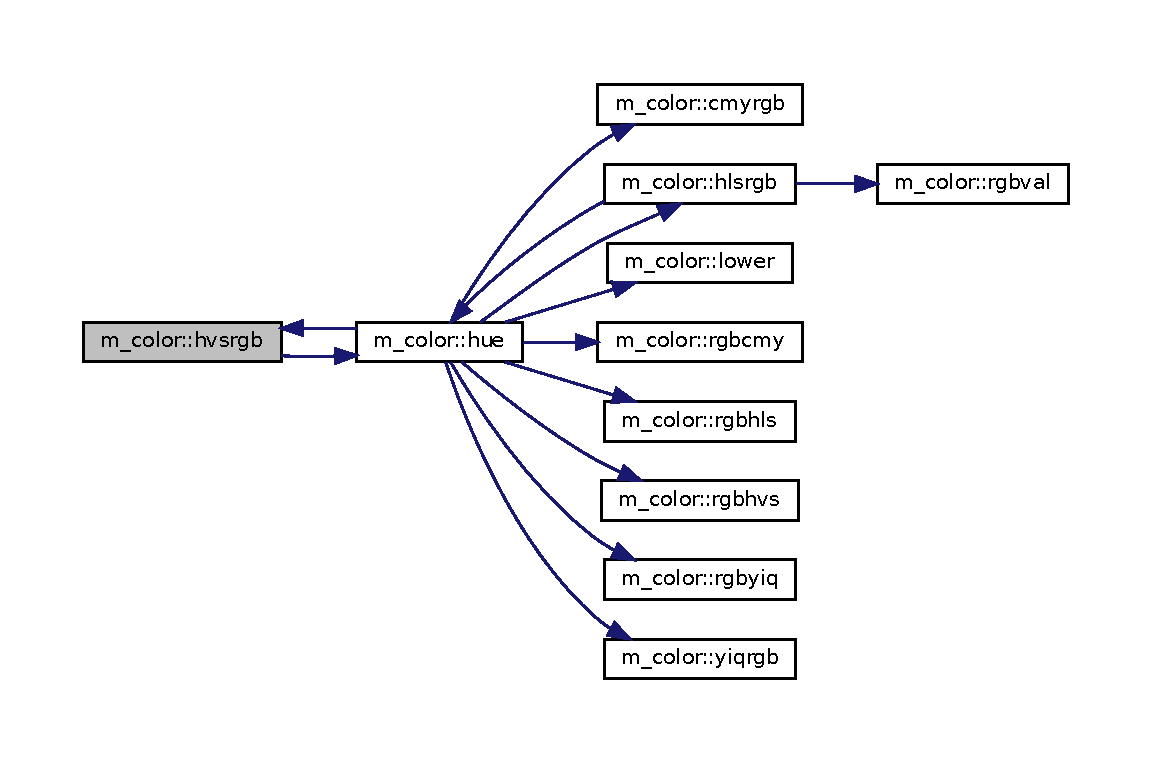
\includegraphics[width=350pt]{namespacem__color_a334ec90d94bbfb9a4c08c5f9efdb8c47_cgraph}
\end{center}
\end{figure}
Here is the caller graph for this function\+:\nopagebreak
\begin{figure}[H]
\begin{center}
\leavevmode
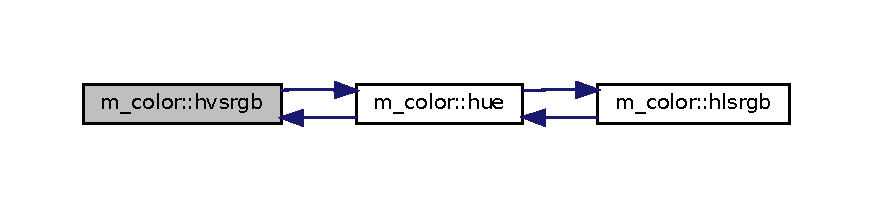
\includegraphics[width=350pt]{namespacem__color_a334ec90d94bbfb9a4c08c5f9efdb8c47_icgraph}
\end{center}
\end{figure}
\mbox{\Hypertarget{namespacem__color_a704e93b42d777a827ec557c92d2dd7dc}\label{namespacem__color_a704e93b42d777a827ec557c92d2dd7dc}} 
\index{m\+\_\+color@{m\+\_\+color}!lower@{lower}}
\index{lower@{lower}!m\+\_\+color@{m\+\_\+color}}
\subsubsection{\texorpdfstring{lower()}{lower()}}
{\footnotesize\ttfamily elemental pure character(len(str)) function m\+\_\+color\+::lower (\begin{DoxyParamCaption}\item[{character($\ast$), intent(in)}]{str }\end{DoxyParamCaption})\hspace{0.3cm}{\ttfamily [private]}}

Here is the caller graph for this function\+:\nopagebreak
\begin{figure}[H]
\begin{center}
\leavevmode
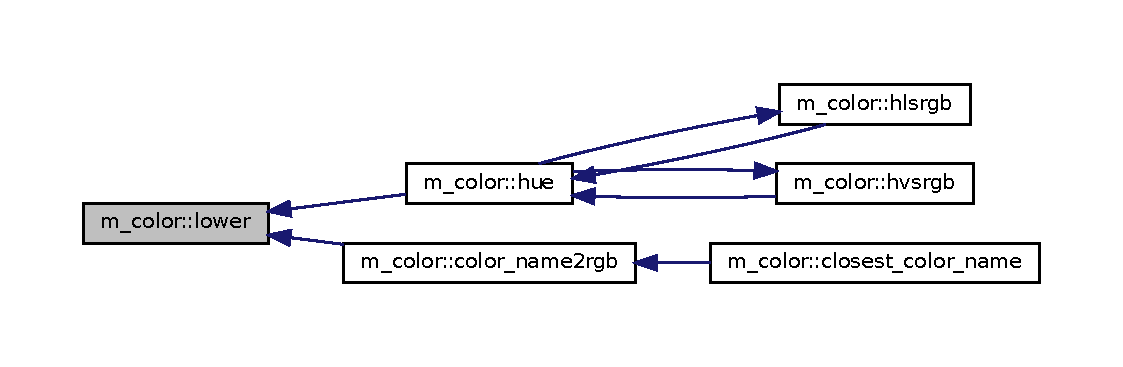
\includegraphics[width=350pt]{namespacem__color_a704e93b42d777a827ec557c92d2dd7dc_icgraph}
\end{center}
\end{figure}
\mbox{\Hypertarget{namespacem__color_ad6e8505eef5add299c4475d289f3c5c5}\label{namespacem__color_ad6e8505eef5add299c4475d289f3c5c5}} 
\index{m\+\_\+color@{m\+\_\+color}!rgbcmy@{rgbcmy}}
\index{rgbcmy@{rgbcmy}!m\+\_\+color@{m\+\_\+color}}
\subsubsection{\texorpdfstring{rgbcmy()}{rgbcmy()}}
{\footnotesize\ttfamily subroutine, private m\+\_\+color\+::rgbcmy (\begin{DoxyParamCaption}\item[{real, intent(in)}]{r,  }\item[{real, intent(in)}]{g,  }\item[{real, intent(in)}]{b,  }\item[{real, intent(out)}]{c,  }\item[{real, intent(out)}]{m,  }\item[{real, intent(out)}]{y,  }\item[{integer}]{status }\end{DoxyParamCaption})\hspace{0.3cm}{\ttfamily [private]}}


\begin{DoxyDescription}
\item[\label{_RGBCMY}%
N\+A\+ME ]rgbcmy(3fp) -\/ \mbox{[}M\+\_\+color\mbox{]} calculates the cyan, magenta, and yellow components given the red, green, and blue component values. (L\+I\+C\+E\+N\+SE\+:PD) 


\item[S\+Y\+N\+O\+P\+S\+IS ]
\begin{DoxyPre}
    subroutine rgbcmy(r,g,b,c,m,y,status)\end{DoxyPre}



\begin{DoxyPre}     ! the red component as a value in the range of 0 to 100
     real, intent(in)  :: r
     ! the green component as a value in the range of 0 to 100
     real, intent(in)  :: g
     ! the blue component as a value in the range of 0 to 100
     real, intent(in)  :: b
     ! the cyan component as a value in the range of 0 to 100
     real, intent(out) :: c
     ! the magenta component as a value in the range of 0 to 100
     real, intent(out) :: m
     ! the yellow component as a value in the range of 0 to 100
     real, intent(out) :: y
     integer           :: status
    \end{DoxyPre}
 


\item[D\+E\+S\+C\+R\+I\+P\+T\+I\+ON ]Table ... ~\newline
~\newline


\begin{quote}
\tabulinesep=1mm
\begin{longtabu} spread 0pt [c]{*{5}{|X[-1]}|}
\hline
\rowcolor{\tableheadbgcolor}\textbf{ Color  }&\textbf{ Color

name  }&\textbf{ (C,M,Y) }&\textbf{ ( R, G, B) }&\textbf{ Hex  }\\\cline{1-5}
\endfirsthead
\hline
\endfoot
\hline
\rowcolor{\tableheadbgcolor}\textbf{ Color  }&\textbf{ Color

name  }&\textbf{ (C,M,Y) }&\textbf{ ( R, G, B) }&\textbf{ Hex  }\\\cline{1-5}
\endhead
~ &Black &(100,100,100) &( 0, 0, 0) &\#000000  \\\cline{1-5}
~ &White &( 0, 0, 0) &(100,100,100) &\#\+F\+F\+F\+F\+FF  \\\cline{1-5}
~ &Red &( 0,100,100) &(100, 0, 0) &\#\+F\+F0000  \\\cline{1-5}
~ &Green &(100, 0,100) &( 0,100, 0) &\#00\+F\+F00  \\\cline{1-5}
~ &Blue &(100,100, 0) &( 0, 0,100) &\#0000\+FF  \\\cline{1-5}
~ &Yellow &( 0, 0,100) &(100,100, 0) &\#\+F\+F\+F\+F00  \\\cline{1-5}
~ &Cyan &(100, 0, 0) &( 0,100,100) &\#00\+F\+F\+FF  \\\cline{1-5}
~ &Magenta &( 0,100, 0) &(100, 0,100) &\#\+F\+F00\+FF  \\\cline{1-5}
\end{longtabu}
\end{quote}





\item[A\+U\+T\+H\+OR ]

John S. Urban




\item[L\+I\+C\+E\+N\+SE ]

Public Domain




\end{DoxyDescription}Here is the caller graph for this function\+:\nopagebreak
\begin{figure}[H]
\begin{center}
\leavevmode
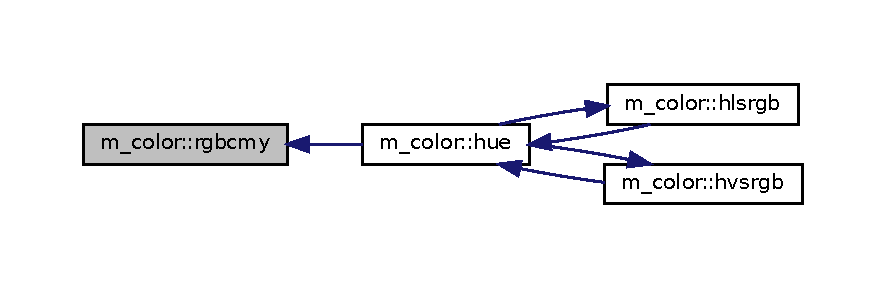
\includegraphics[width=350pt]{namespacem__color_ad6e8505eef5add299c4475d289f3c5c5_icgraph}
\end{center}
\end{figure}
\mbox{\Hypertarget{namespacem__color_a1dd027cbe65112af243d26195b1fc49a}\label{namespacem__color_a1dd027cbe65112af243d26195b1fc49a}} 
\index{m\+\_\+color@{m\+\_\+color}!rgbhls@{rgbhls}}
\index{rgbhls@{rgbhls}!m\+\_\+color@{m\+\_\+color}}
\subsubsection{\texorpdfstring{rgbhls()}{rgbhls()}}
{\footnotesize\ttfamily subroutine, private m\+\_\+color\+::rgbhls (\begin{DoxyParamCaption}\item[{real}]{r0,  }\item[{real}]{g0,  }\item[{real}]{b0,  }\item[{real}]{h,  }\item[{real}]{l,  }\item[{real}]{s,  }\item[{integer}]{status }\end{DoxyParamCaption})\hspace{0.3cm}{\ttfamily [private]}}


\begin{DoxyDescription}
\item[\label{_RGBHLS}%
N\+A\+ME ]R\+G\+B\+H\+L\+S(3fp) -\/ \mbox{[}M\+\_\+color\mbox{]} Given red, green, and blue color components calculates the hue, lightness, and saturation for a color (L\+I\+C\+E\+N\+SE\+:PD) 


\item[S\+Y\+N\+O\+P\+S\+IS ]
\begin{DoxyPre}\end{DoxyPre}



\begin{DoxyPre}    subroutine rgbhls(r,g,b,h,l,s,status)\end{DoxyPre}



\begin{DoxyPre}     ! red component as a value of 0 to 100
     real, intent(in)  :: r
     ! green component as a value of 0 to 100
     real, intent(in)  :: g
     ! blue component as a value of 0 to 100
     real, intent(in)  :: b
     ! hue value in the range of 0 to 360 degrees
     real, intent(out) :: h
     ! lightness as a percent value from 0 to 100
     real, intent(out) :: l
     ! saturation as a percent from 0 to 100
     real, intent(out) :: s
     integer           :: status
    \end{DoxyPre}
 


\item[D\+E\+S\+C\+R\+I\+P\+T\+I\+ON ]

R\+GB values are in the range 0-\/100; hue is 0-\/360 degrees; lightness and saturation have a range of 0-\/100. ~\newline
~\newline


\begin{quote}
\tabulinesep=1mm
\begin{longtabu} spread 0pt [c]{*{8}{|X[-1]}|}
\hline
\rowcolor{\tableheadbgcolor}\textbf{ Color}&\multicolumn{3}{p{(\linewidth-\tabcolsep*8-\arrayrulewidth*4)*3/8}|}{\cellcolor{\tableheadbgcolor}\textbf{ R\+GB}}&\multicolumn{3}{p{(\linewidth-\tabcolsep*8-\arrayrulewidth*4)*3/8}|}{\cellcolor{\tableheadbgcolor}\textbf{ H\+LS}}&\textbf{ Sample }\\\cline{1-8}
\endfirsthead
\hline
\endfoot
\hline
\rowcolor{\tableheadbgcolor}\textbf{ Color}&\multicolumn{3}{p{(\linewidth-\tabcolsep*8-\arrayrulewidth*4)*3/8}|}{\cellcolor{\tableheadbgcolor}\textbf{ R\+GB}}&\multicolumn{3}{p{(\linewidth-\tabcolsep*8-\arrayrulewidth*4)*3/8}|}{\cellcolor{\tableheadbgcolor}\textbf{ H\+LS}}&\textbf{ Sample }\\\cline{1-8}
\endhead
Red&100.\+0&0.\+0&0.\+0&0&50.\+0&100.\+0&~ \\\cline{1-8}
Yellow&100.\+0&100.\+0&0.\+0&60&50.\+0&100.\+0&~ \\\cline{1-8}
Green&0.\+0&100.\+0&0.\+0&120&50.\+0&100.\+0&~ \\\cline{1-8}
Cyan&0.\+0&100.\+0&100.\+0&180&50.\+0&100.\+0&~ \\\cline{1-8}
Blue&0.\+0&0.\+0&100.\+0&240&50.\+0&100.\+0&~ \\\cline{1-8}
Magenta&100.\+0&0.\+0&100.\+0&300&50.\+0&100.\+0&~ \\\cline{1-8}
White&100.\+0&100.\+0&100.\+0&(any)&100.\+0&(any)&~ \\\cline{1-8}
Black&0.\+0&0.\+0&0.\+0&(any)&0.\+0&(any)&~ \\\cline{1-8}
Maroon&50.\+0&0.\+0&0.\+0&0&25.\+0&100.\+0&~ \\\cline{1-8}
Pink&100.\+0&50.\+0&50.\+0&0&75.\+0&100.\+0&~ \\\cline{1-8}
\end{longtabu}
\end{quote}



\item[A\+U\+T\+H\+OR ]

John S. Urban




\item[L\+I\+C\+E\+N\+SE ]

Public Domain




\end{DoxyDescription}Here is the caller graph for this function\+:\nopagebreak
\begin{figure}[H]
\begin{center}
\leavevmode
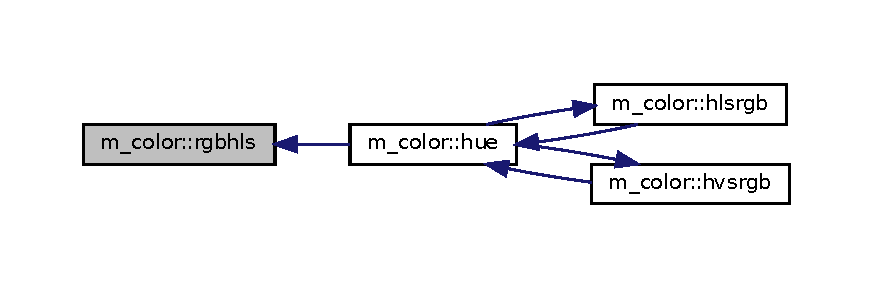
\includegraphics[width=350pt]{namespacem__color_a1dd027cbe65112af243d26195b1fc49a_icgraph}
\end{center}
\end{figure}
\mbox{\Hypertarget{namespacem__color_a76f00e1d418c4904a963094bc730a0e6}\label{namespacem__color_a76f00e1d418c4904a963094bc730a0e6}} 
\index{m\+\_\+color@{m\+\_\+color}!rgbhvs@{rgbhvs}}
\index{rgbhvs@{rgbhvs}!m\+\_\+color@{m\+\_\+color}}
\subsubsection{\texorpdfstring{rgbhvs()}{rgbhvs()}}
{\footnotesize\ttfamily subroutine, private m\+\_\+color\+::rgbhvs (\begin{DoxyParamCaption}\item[{real, intent(in)}]{r0,  }\item[{real, intent(in)}]{g0,  }\item[{real, intent(in)}]{b0,  }\item[{real, intent(out)}]{h,  }\item[{real, intent(out)}]{v,  }\item[{real, intent(out)}]{s,  }\item[{integer}]{status }\end{DoxyParamCaption})\hspace{0.3cm}{\ttfamily [private]}}


\begin{DoxyDescription}
\item[\label{_RGBHVS}%
N\+A\+ME ]R\+G\+B\+H\+V\+S(3fp) -\/ \mbox{[}M\+\_\+color\mbox{]} calculates the hue, value, \& saturation for a color given in red, green, \& blue components values. (L\+I\+C\+E\+N\+SE\+:PD) 


\item[S\+Y\+N\+O\+P\+S\+IS ]
\begin{DoxyPre}
    subroutine rgbhvs(r,g,b,h,v,s,status)\end{DoxyPre}



\begin{DoxyPre}     ! the red component as a value of 0 to 100.
     real, intent(in)  :: r
     ! the green component as a value of 0 to 100.
     real, intent(in)  :: g
     ! the blue component as a value of 0 to 100.
     real, intent(in)  :: b
     ! the hue value in the range of 0 to 360 degrees
     real, intent(out) :: h
     ! the "value" as a percent value from 0 to 100.
     real, intent(out) :: v
     ! the saturation as a percent from 0 to 100.
     real, intent(out) :: s
     integer           :: status
    
\begin{DoxyPre}
 \end{DoxyPre}
\end{DoxyPre}



\begin{DoxyPre}
\begin{DoxyPre} \end{DoxyPre}
\end{DoxyPre}

\item[D\+E\+S\+C\+R\+I\+P\+T\+I\+ON ]
\begin{DoxyPre}
\begin{DoxyPre}\end{DoxyPre}
\end{DoxyPre}



\begin{DoxyPre}
\begin{DoxyPre} RGBHVS() calculates the hue, value, \& saturation
 for a color given in red, green, \& blue components values.
 ~\newline
~\newline
\end{DoxyPre}
\end{DoxyPre}



\begin{DoxyPre}
\begin{DoxyPre} \begin{quote}
\tabulinesep=1mm
\begin{longtabu} spread 0pt [c]{*{5}{|X[-1]}|}
\hline
\rowcolor{\tableheadbgcolor}\textbf{ Color  }&\textbf{ Color~\newline
name }&\textbf{ Hex      }&\textbf{ (R,G,B)        }&\textbf{ (H,S,V)                  
 }\\\cline{1-5}
\endfirsthead
\hline
\endfoot
\hline
\rowcolor{\tableheadbgcolor}\textbf{ Color  }&\textbf{ Color~\newline
name }&\textbf{ Hex      }&\textbf{ (R,G,B)        }&\textbf{ (H,S,V)                  
 }\\\cline{1-5}
\endhead
~  &Black         &\#000000  &(0,0,0)        &(0\textordmasculine{},0\%,0\%)        
 \\\cline{1-5}
~  &White         &#FFFFFF  &(100,100,100)  &(0\textordmasculine{},0\%,100\%)      
 \\\cline{1-5}
~  &Red           &#FF0000  &(100,0,0)      &(0\textordmasculine{},100\%,100\%)    
 \\\cline{1-5}
~  &Lime          &\#00FF00  &(0,100,0)      &(120\textordmasculine{},100\%,100\%)  
 \\\cline{1-5}
~  &Blue          &\#0000FF  &(0,0,100)      &(240\textordmasculine{},100\%,100\%)  
 \\\cline{1-5}
~  &Yellow        &#FFFF00  &(100,100,0)    &(60\textordmasculine{},100\%,100\%)   
 \\\cline{1-5}
~  &Cyan          &\#00FFFF  &(0,100,100)    &(180\textordmasculine{},100\%,100\%)  
 \\\cline{1-5}
~  &Magenta       &#FF00FF  &(100,0,100)    &(300\textordmasculine{},100\%,100\%)  
 \\\cline{1-5}
~  &Silver        &#C0C0C0  &(75,75,75)     &(0\textordmasculine{},0\%,75\%)       
 \\\cline{1-5}
~  &Gray          &\#808080  &(50,50,50)     &(0\textordmasculine{},0\%,50\%)       
 \\\cline{1-5}
~  &Maroon        &\#800000  &(50,0,0)       &(0\textordmasculine{},100\%,50\%)     
 \\\cline{1-5}
~  &Olive         &\#808000  &(50,50,0)      &(60\textordmasculine{},100\%,50\%)    
 \\\cline{1-5}
~  &Green         &\#008000  &(0,50,0)       &(120\textordmasculine{},100\%,50\%)   
 \\\cline{1-5}
~  &Purple        &\#800080  &(50,0,50)      &(300\textordmasculine{},100\%,50\%)   
 \\\cline{1-5}
~  &Teal          &\#008080  &(0,50,50)      &(180\textordmasculine{},100\%,50\%)   
 \\\cline{1-5}
~  &Navy          &\#000080  &(0,0,50)       &(240\textordmasculine{},100\%,50\%)     
 \\\cline{1-5}
\end{longtabu}
\end{quote}
\end{DoxyPre}
\end{DoxyPre}



\begin{DoxyPre}
\begin{DoxyPre} \end{DoxyPre}
\end{DoxyPre}

\item[A\+U\+T\+H\+OR ]
\begin{DoxyPre}
\begin{DoxyPre}\end{DoxyPre}
\end{DoxyPre}



\begin{DoxyPre}
\begin{DoxyPre}    John S. Urban\end{DoxyPre}
\end{DoxyPre}



\begin{DoxyPre}
\begin{DoxyPre} \end{DoxyPre}
\end{DoxyPre}



\begin{DoxyPre}
\begin{DoxyPre} \end{DoxyPre}
\end{DoxyPre}

\item[L\+I\+C\+E\+N\+SE ]
\begin{DoxyPre}
\begin{DoxyPre}\end{DoxyPre}
\end{DoxyPre}



\begin{DoxyPre}
\begin{DoxyPre}    Public Domain\end{DoxyPre}
\end{DoxyPre}



\begin{DoxyPre}
\begin{DoxyPre} \end{DoxyPre}
\end{DoxyPre}



\begin{DoxyPre}
\begin{DoxyPre} \end{DoxyPre}
\end{DoxyPre}

\end{DoxyDescription}Here is the caller graph for this function\+:\nopagebreak
\begin{figure}[H]
\begin{center}
\leavevmode
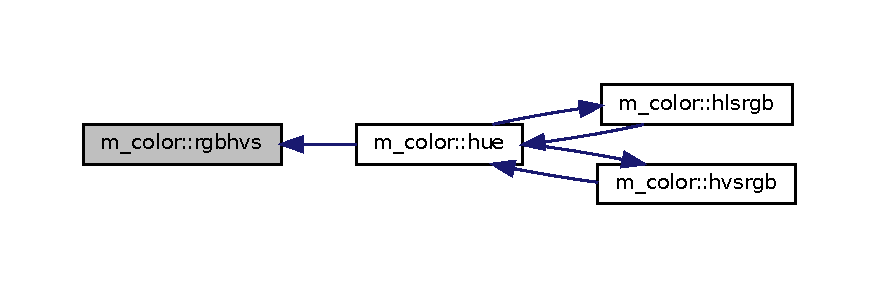
\includegraphics[width=350pt]{namespacem__color_a76f00e1d418c4904a963094bc730a0e6_icgraph}
\end{center}
\end{figure}
\mbox{\Hypertarget{namespacem__color_aca19999686fc20d79da580c6a643dc35}\label{namespacem__color_aca19999686fc20d79da580c6a643dc35}} 
\index{m\+\_\+color@{m\+\_\+color}!rgbmono@{rgbmono}}
\index{rgbmono@{rgbmono}!m\+\_\+color@{m\+\_\+color}}
\subsubsection{\texorpdfstring{rgbmono()}{rgbmono()}}
{\footnotesize\ttfamily subroutine, public m\+\_\+color\+::rgbmono (\begin{DoxyParamCaption}\item[{real, intent(in)}]{rr,  }\item[{real, intent(in)}]{rg,  }\item[{real, intent(in)}]{rb,  }\item[{real, intent(out)}]{ri,  }\item[{integer, intent(out)}]{status }\end{DoxyParamCaption})}



\subsubsection*{N\+A\+ME}

R\+G\+B\+M\+O\+N\+O(3f) -\/ \mbox{[}M\+\_\+color\mbox{]} converts R\+GB colors to a reasonable grayscale intensity (L\+I\+C\+E\+N\+SE\+:PD) 

\subsubsection*{S\+Y\+N\+O\+P\+S\+IS}

\begin{DoxyVerb}subroutine rgbmono</a>(rr,rg,rb,ri,status)

 real, intent(in)  :: RR
 real, intent(in)  :: RG
 real, intent(in)  :: RB
 real, intent(out) :: RI
 integer           :: status
\end{DoxyVerb}


\subsubsection*{D\+E\+S\+C\+R\+I\+P\+T\+I\+ON}

R\+G\+B\+M\+O\+N\+O(3f) converts R\+GB colors to a reasonable grayscale intensity. This can be used to produce monochrome images from color images. Intensity is calculated from the specified Red, Green, Blue intensities as 0.\+30$\ast$R + 0.\+59$\ast$G + 0.\+11$\ast$B, as in U.\+S. color television systems, N\+T\+SC encoding. Note that most devices do not have an infinite range of monochrome intensities available.

\subsubsection*{O\+P\+T\+I\+O\+NS}

RR red component of the input color in the range 0 to 100 RG green component of the input color in the range 0 to 100 RB blue component of the input color in the range 0 to 100

\subsubsection*{R\+E\+T\+U\+R\+NS}

RI grayscale intensity calculated in the range 0 to 100 status zero (0) if no error occurred, otherwise result is out of bounds

\subsubsection*{E\+X\+A\+M\+P\+L\+ES}

Sample\+:

program demo\+\_\+rgbmono use M\+\_\+color, only \+: rgbmono implicit none real \+:\+: gray integer \+:\+: ierr call rgbmono(100.\+0, 0.\+0, 0.\+0,gray,ierr); write($\ast$,$\ast$)\textquotesingle{}red \textquotesingle{},gray call rgbmono( 0.\+0,100.\+0, 0.\+0,gray,ierr); write($\ast$,$\ast$)\textquotesingle{}green \textquotesingle{},gray call rgbmono( 0.\+0, 0.\+0,100.\+0,gray,ierr); write($\ast$,$\ast$)\textquotesingle{}blue \textquotesingle{},gray call rgbmono(100.\+0,100.\+0, 0.\+0,gray,ierr); write($\ast$,$\ast$)\textquotesingle{}Yellow \textquotesingle{},gray call rgbmono( 0.\+0,100.\+0,100.\+0,gray,ierr); write($\ast$,$\ast$)\textquotesingle{}Cyan \textquotesingle{},gray call rgbmono(100.\+0, 0.\+0,100.\+0,gray,ierr); write($\ast$,$\ast$)\textquotesingle{}Magenta \textquotesingle{},gray call rgbmono(100.\+0,100.\+0,100.\+0,gray,ierr); write($\ast$,$\ast$)\textquotesingle{}White \textquotesingle{},gray call rgbmono( 00.\+0, 0.\+0, 0.\+0,gray,ierr); write($\ast$,$\ast$)\textquotesingle{}Black \textquotesingle{},gray call rgbmono( 50.\+0, 0.\+0, 0.\+0,gray,ierr); write($\ast$,$\ast$)\textquotesingle{}Maroon \textquotesingle{},gray call rgbmono(100.\+0, 50.\+0, 50.\+0,gray,ierr); write($\ast$,$\ast$)\textquotesingle{}Pink \textquotesingle{},gray end program demo\+\_\+rgbmono

Results\+:

red 30.\+0000019 green 58.\+9999962 blue 11.\+0000000 Yellow 89.\+0000000 Cyan 70.\+0000000 Magenta 41.\+0000000 White 100.\+000000 Black 0.\+00000000 Maroon 15.\+0000010 Pink 65.\+0000000

\subsubsection*{A\+U\+T\+H\+OR}

John S. Urban

\subsubsection*{L\+I\+C\+E\+N\+SE}

Public Domain \mbox{\Hypertarget{namespacem__color_a3e97e24dba7b820f685f13eaa64a6caa}\label{namespacem__color_a3e97e24dba7b820f685f13eaa64a6caa}} 
\index{m\+\_\+color@{m\+\_\+color}!rgbval@{rgbval}}
\index{rgbval@{rgbval}!m\+\_\+color@{m\+\_\+color}}
\subsubsection{\texorpdfstring{rgbval()}{rgbval()}}
{\footnotesize\ttfamily real function, private m\+\_\+color\+::rgbval (\begin{DoxyParamCaption}\item[{real}]{clr1,  }\item[{real}]{clr2,  }\item[{real}]{h }\end{DoxyParamCaption})\hspace{0.3cm}{\ttfamily [private]}}


\begin{DoxyDescription}
\item[\label{_RGBVAL}%
N\+A\+ME ]R\+G\+B\+V\+A\+L(3fp) -\/ \mbox{[}M\+\_\+color\mbox{]} is an internal private function used by hlsrgb(3fp). (L\+I\+C\+E\+N\+SE\+:PD) 


\item[S\+Y\+N\+O\+P\+S\+IS]
\begin{DoxyPre}
    subroutine rgbval(clr1,clr2,h)\end{DoxyPre}



\begin{DoxyPre}     integer, intent(in) :: h ! H is the hue value in degrees
     real, intent(in) :: clr1 !
     real, intent(in) :: clr2 !
    \end{DoxyPre}
 


\item[D\+E\+S\+C\+R\+I\+P\+T\+I\+ON ]Function R\+G\+B\+V\+A\+L(3f) is an internal private function used by \mbox{\hyperlink{namespacem__color_a40e6c91da216384eded2157cdaf86eba}{hlsrgb()}}.




\item[A\+U\+T\+H\+OR ]

John S. Urban




\item[L\+I\+C\+E\+N\+SE ]

Public Domain




\end{DoxyDescription}Here is the caller graph for this function\+:\nopagebreak
\begin{figure}[H]
\begin{center}
\leavevmode
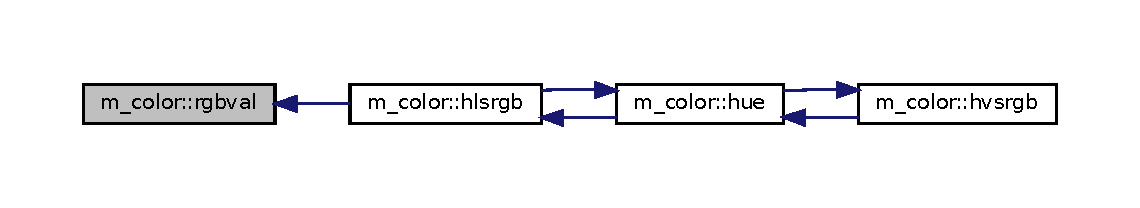
\includegraphics[width=350pt]{namespacem__color_a3e97e24dba7b820f685f13eaa64a6caa_icgraph}
\end{center}
\end{figure}
\mbox{\Hypertarget{namespacem__color_a386d004a1392b7e01ff66f1676d43def}\label{namespacem__color_a386d004a1392b7e01ff66f1676d43def}} 
\index{m\+\_\+color@{m\+\_\+color}!rgbyiq@{rgbyiq}}
\index{rgbyiq@{rgbyiq}!m\+\_\+color@{m\+\_\+color}}
\subsubsection{\texorpdfstring{rgbyiq()}{rgbyiq()}}
{\footnotesize\ttfamily subroutine, private m\+\_\+color\+::rgbyiq (\begin{DoxyParamCaption}\item[{real, intent(in)}]{r,  }\item[{real, intent(in)}]{g,  }\item[{real, intent(in)}]{b,  }\item[{real, intent(out)}]{y,  }\item[{real, intent(out)}]{i,  }\item[{real, intent(out)}]{q,  }\item[{integer}]{status }\end{DoxyParamCaption})\hspace{0.3cm}{\ttfamily [private]}}


\begin{DoxyDescription}
\item[\label{_RGBYIQ}%
N\+A\+ME ]R\+G\+B\+Y\+I\+Q(3fp) -\/ \mbox{[}M\+\_\+color\mbox{]} Convert R\+GB values to luma, orange-\/blue chrominance, and purple-\/green chrominance. (L\+I\+C\+E\+N\+SE\+:PD) 


\item[S\+Y\+N\+O\+P\+S\+IS ]
\begin{DoxyPre}
    subroutine rgbyiq(r,g,b,y,i,q,status)\end{DoxyPre}



\begin{DoxyPre}     real,intent(in)  :: r,g,b
     real,intent(out) :: y,i,q
     integer          :: status
    \end{DoxyPre}
 


\item[D\+E\+S\+C\+R\+I\+P\+T\+I\+ON ]Convert R\+GB values to luma, orange-\/blue chrominance, and purple-\/green chrominance. 


\item[A\+U\+T\+H\+OR ]

John S. Urban




\item[L\+I\+C\+E\+N\+SE ]

Public Domain




\end{DoxyDescription}Here is the caller graph for this function\+:\nopagebreak
\begin{figure}[H]
\begin{center}
\leavevmode
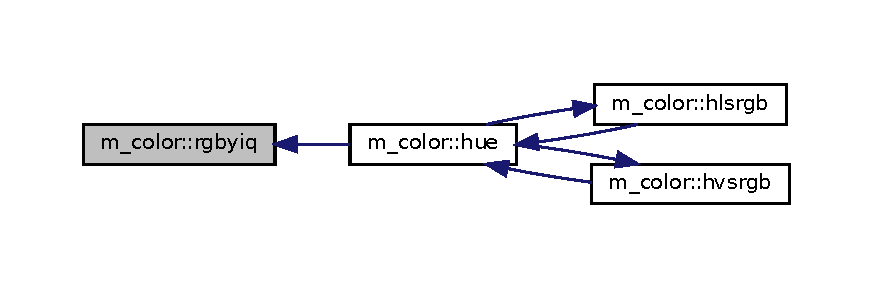
\includegraphics[width=350pt]{namespacem__color_a386d004a1392b7e01ff66f1676d43def_icgraph}
\end{center}
\end{figure}
\mbox{\Hypertarget{namespacem__color_ac9cd845fb9975144a6deb3a21ce29a29}\label{namespacem__color_ac9cd845fb9975144a6deb3a21ce29a29}} 
\index{m\+\_\+color@{m\+\_\+color}!yiqrgb@{yiqrgb}}
\index{yiqrgb@{yiqrgb}!m\+\_\+color@{m\+\_\+color}}
\subsubsection{\texorpdfstring{yiqrgb()}{yiqrgb()}}
{\footnotesize\ttfamily subroutine m\+\_\+color\+::yiqrgb (\begin{DoxyParamCaption}\item[{real, intent(in)}]{y,  }\item[{real, intent(in)}]{i,  }\item[{real, intent(in)}]{q,  }\item[{real, intent(out)}]{r,  }\item[{real, intent(out)}]{g,  }\item[{real, intent(out)}]{b,  }\item[{integer}]{status }\end{DoxyParamCaption})\hspace{0.3cm}{\ttfamily [private]}}


\begin{DoxyDescription}
\item[\label{_YIQRGB}%
N\+A\+ME ]Y\+I\+Q\+R\+G\+B(3fp) -\/ \mbox{[}M\+\_\+color\mbox{]} Convert luma, orange-\/blue chrominance, and purple-\/green chrominance to R\+GB values. (L\+I\+C\+E\+N\+SE\+:PD) 


\item[S\+Y\+N\+O\+P\+S\+IS ]
\begin{DoxyPre}
    subroutine yiqrgb(y,i,q,r,g,b,status)\end{DoxyPre}



\begin{DoxyPre}     real,intent(in)  :: y,i,q
     real,intent(out) :: r,g,b
     integer          :: status
    \end{DoxyPre}
 


\item[D\+E\+S\+C\+R\+I\+P\+T\+I\+ON ]

Convert luma, orange-\/blue chrominance, and purple-\/green chrominance to R\+GB values.




\item[A\+U\+T\+H\+OR ]

John S. Urban




\item[L\+I\+C\+E\+N\+SE ]

Public Domain




\end{DoxyDescription}Here is the caller graph for this function\+:\nopagebreak
\begin{figure}[H]
\begin{center}
\leavevmode
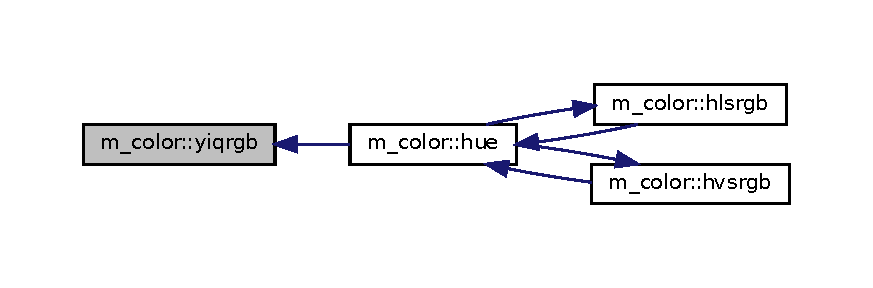
\includegraphics[width=350pt]{namespacem__color_ac9cd845fb9975144a6deb3a21ce29a29_icgraph}
\end{center}
\end{figure}

\chapter{File Documentation}
\hypertarget{M__color_8f90}{}\section{/home/urbanjs/venus/\+V600/github/\+M\+\_\+color/src/\+M\+\_\+color.f90 File Reference}
\label{M__color_8f90}\index{/home/urbanjs/venus/\+V600/github/\+M\+\_\+color/src/\+M\+\_\+color.\+f90@{/home/urbanjs/venus/\+V600/github/\+M\+\_\+color/src/\+M\+\_\+color.\+f90}}
\subsection*{Modules}
\begin{DoxyCompactItemize}
\item 
module \mbox{\hyperlink{namespacem__color}{m\+\_\+color}}
\end{DoxyCompactItemize}
\subsection*{Functions/\+Subroutines}
\begin{DoxyCompactItemize}
\item 
subroutine, public \mbox{\hyperlink{namespacem__color_a56dd07bbf1378ccc78a230d171f9d429}{m\+\_\+color\+::hue}} (modei, clr1i, clr2i, clr3i, modeo, clr1o, clr2o, clr3o, status)
\item 
subroutine, private \mbox{\hyperlink{namespacem__color_a1dd027cbe65112af243d26195b1fc49a}{m\+\_\+color\+::rgbhls}} (r0, g0, b0, h, l, s, status)
\item 
subroutine, private \mbox{\hyperlink{namespacem__color_a76f00e1d418c4904a963094bc730a0e6}{m\+\_\+color\+::rgbhvs}} (r0, g0, b0, h, v, s, status)
\item 
subroutine, private \mbox{\hyperlink{namespacem__color_ab91687e87d0901874e52efe5933e3044}{m\+\_\+color\+::cmyrgb}} (c, m, y, r, g, b, status)
\item 
subroutine, private \mbox{\hyperlink{namespacem__color_ad6e8505eef5add299c4475d289f3c5c5}{m\+\_\+color\+::rgbcmy}} (r, g, b, c, m, y, status)
\item 
subroutine, public \mbox{\hyperlink{namespacem__color_aca19999686fc20d79da580c6a643dc35}{m\+\_\+color\+::rgbmono}} (rr, rg, rb, ri, status)
\begin{DoxyCompactList}\small\item\em \subsubsection*{N\+A\+ME}

R\+G\+B\+M\+O\+N\+O(3f) -\/ \mbox{[}M\+\_\+color\mbox{]} converts R\+GB colors to a reasonable grayscale intensity. (L\+I\+C\+E\+N\+SE\+:PD) \end{DoxyCompactList}\item 
real function, private \mbox{\hyperlink{namespacem__color_a3e97e24dba7b820f685f13eaa64a6caa}{m\+\_\+color\+::rgbval}} (clr1, clr2, h)
\item 
subroutine, private \mbox{\hyperlink{namespacem__color_a40e6c91da216384eded2157cdaf86eba}{m\+\_\+color\+::hlsrgb}} (H, L, S, R, G, B, status)
\item 
subroutine, private \mbox{\hyperlink{namespacem__color_a334ec90d94bbfb9a4c08c5f9efdb8c47}{m\+\_\+color\+::hvsrgb}} (h, v, s, r, g, b, status)
\item 
subroutine \mbox{\hyperlink{namespacem__color_ac9cd845fb9975144a6deb3a21ce29a29}{m\+\_\+color\+::yiqrgb}} (y, i, q, r, g, b, status)
\item 
subroutine, private \mbox{\hyperlink{namespacem__color_a386d004a1392b7e01ff66f1676d43def}{m\+\_\+color\+::rgbyiq}} (r, g, b, y, i, q, status)
\item 
subroutine, public \mbox{\hyperlink{namespacem__color_acad72628ee0b77cf87f40cd46734fb18}{m\+\_\+color\+::closest\+\_\+color\+\_\+name}} (r, g, b, closestname)
\begin{DoxyCompactList}\small\item\em \subsubsection*{N\+A\+ME}

closest\+\_\+color\+\_\+name(3f) -\/ \mbox{[}M\+\_\+color\mbox{]} returns the closest name for the given R\+GB values. (L\+I\+C\+E\+N\+SE\+:PD) \subsubsection*{S\+Y\+N\+O\+P\+S\+IS}\end{DoxyCompactList}\item 
subroutine, public \mbox{\hyperlink{namespacem__color_a84a36043d278bc56a7148483a862dec8}{m\+\_\+color\+::color\+\_\+name2rgb}} (name, r, g, b, echoname)
\begin{DoxyCompactList}\small\item\em \subsubsection*{N\+A\+ME}

C\+O\+L\+O\+R\+\_\+\+N\+A\+M\+E2\+R\+G\+B(3f) -\/ \mbox{[}M\+\_\+color\mbox{]} returns the R\+GB values in the range 0 to 100 for a given known color name. (L\+I\+C\+E\+N\+SE\+:PD) \subsubsection*{S\+Y\+N\+O\+P\+S\+IS}\end{DoxyCompactList}\item 
elemental pure character(len(str)) function \mbox{\hyperlink{namespacem__color_a704e93b42d777a827ec557c92d2dd7dc}{m\+\_\+color\+::lower}} (str)
\end{DoxyCompactItemize}

\hypertarget{mainpage_8txt}{}\section{/home/urbanjs/venus/\+V600/github/\+M\+\_\+color/src/mainpage.txt File Reference}
\label{mainpage_8txt}\index{/home/urbanjs/venus/\+V600/github/\+M\+\_\+color/src/mainpage.\+txt@{/home/urbanjs/venus/\+V600/github/\+M\+\_\+color/src/mainpage.\+txt}}

%--- End generated contents ---

% Index
\backmatter
\newpage
\phantomsection
\clearemptydoublepage
\addcontentsline{toc}{chapter}{Index}
\printindex

\end{document}
